\documentclass[]{article}
\usepackage[ngerman]{babel}
\usepackage[utf8]{inputenc}
\usepackage{amssymb}
\usepackage{amsmath}
\usepackage[all]{xy}
\usepackage{graphics,color} 
\usepackage{graphicx}
\usepackage{multicol}
\usepackage[ngerman]{varioref}
\usepackage{float}
\usepackage{amsthm}
\newtheorem{Definition}{Definition}
\newtheorem{Beispiel}{Beispiel}
\newtheorem{Satz}{Satz}
\newtheorem{Bemerkung}{Bemerkung}

\newtheorem{Algorithmus}{Algorithmus}


\usepackage{ifthen}
\providecommand{\IfDefined}[2]{%
    \ifcsname #1\endcsname
    #2 %
    \else
    % do nothing
    \fi
}

\providecommand{\IfElseDefined}[3]{%
    \ifcsname #1\endcsname
    #2 %
    \else
    #3 %
    \fi
}

\begin{document}
%front
\title{Einführung in die Computergrafik}
\author{Johannes Riesterer}
\date{\today}
\maketitle\thispagestyle{empty}
\newpage 
\begin{center}
\large
 \copyright Johannes Riesterer \\
Vervielfältigung nur mit ausdrücklicher Erlaubnis des Autors
\end{center}
\thispagestyle{empty}
\newpage

\section*{Vorwort}

\mbox{}\thispagestyle{empty}
\newpage

\tableofcontents
\mbox{}\thispagestyle{empty}
\newpage
%main
\section{Mathematische Werkzeuge}

\subsection{Lineare Algebra}
\subsubsection{Vektoren und Matrizen}
Wir wollen zunächst  den Vektorraum $\mathbb{R}^n$ einführen. Hierbei ist $n$ eigentlich immer $2,3$ oder $4$.
Zunächst ist der $\mathbb{R}^n$  eine Menge, nämlich die Menge der $n$-dimensionalen Vektoren 
\begin{align*}
\mathbb{R}^n : = \Biggl \{
\begin{pmatrix}
x_1 \\ x_2 \\ \vdots \\ x_n
\end{pmatrix} \Bigg | \; x_1, x_2, \hdots ,x_n \in \mathbb{R}
 \Biggr \}  \; .
\end{align*}
Auf dieser Menge der Vektoren definiert man die Addition
\begin{align*}
+ : \mathbb{R}^n \times  \mathbb{R}^n   & \to \mathbb{R}^n \\
\begin{pmatrix}
x_1 \\ x_2 \\ \vdots \\ x_n
\end{pmatrix}  +  
\begin{pmatrix}
y_1 \\ y_2 \\ \vdots \\ y_n
\end{pmatrix} 
&  :=  \begin{pmatrix}
x_1 + y_1 \\ x_2  + y_2 \\ \vdots \\ x_n + y_n
\end{pmatrix} 
\end{align*}

und die sogenannte Skalarmultiplikation 
\begin{align*}
\cdot : \mathbb{R} \times  \mathbb{R}^n   & \to \mathbb{R}^n \\
\lambda \cdot \begin{pmatrix}
x_1 \\ x_2 \\ \vdots \\ x_n
\end{pmatrix}  
&  :=  \begin{pmatrix}
\lambda  \cdot x_1  \\  \lambda \cdot x_2 \\ \vdots \\  \lambda \cdot x_n 
\end{pmatrix} \; . 
\end{align*}
Das Element $\lambda  \in \mathbb{R}$ nennt man auch Skalar.
\begin{Definition}
Der Vektorraum $\mathbb{R}^n$ ist das Tripel 
$(\mathbb{R}^n, + , \cdot )$.
\end{Definition}

\begin{Beispiel}
\begin{align*}
\begin{pmatrix}
1 \\ 2  \\  3
\end{pmatrix}  +  
\begin{pmatrix}
3 \\ 2  \\ 1
\end{pmatrix} 
=  \begin{pmatrix}
4 \\ 4  \\ 4
\end{pmatrix} 
\end{align*}

\begin{align*}
\begin{pmatrix}
 1 \\  1 
\end{pmatrix}  +  
\begin{pmatrix}
-1  \\  -1 
\end{pmatrix} 
=  \begin{pmatrix}
0  \\  0 
\end{pmatrix}  
\end{align*}

\begin{align*}
\begin{pmatrix}
1 \\ -1  \\  -\frac{1}{2}  \\ 2 
\end{pmatrix}  +  
\begin{pmatrix}
0  \\  0 \\  0 \\ 0
\end{pmatrix} 
=  \begin{pmatrix}
1 \\ -1  \\  -\frac{1}{2}  \\ 2 
\end{pmatrix} 
\end{align*}

\begin{align*}
-1 \cdot
\begin{pmatrix}
1 \\ 1  \\  1 
\end{pmatrix}  
=  \begin{pmatrix}
-1   \\ -  1    \\  -1  
\end{pmatrix} 
\end{align*}

 
\begin{align*}
\pi \cdot
\begin{pmatrix}
1 \\ 2  \\  3 \\ 4
\end{pmatrix}  
=  \begin{pmatrix}
\pi   \\ 2  \pi  \\  3 \pi \\  4  \pi
\end{pmatrix} 
\end{align*}

\begin{Bemerkung}
Für alle Skalare $\lambda, \mu \in \mathbb{R}$ und Vektoren $u,v \in  \mathbb{R}^n$ gelten die  Rechenregeln
\begin{align*}
\lambda \cdot (u +v) = \lambda \cdot u + \lambda \cdot v \\
(\lambda + \mu)  \cdot u  = \lambda  \cdot u + \mu  \cdot u \; .
\end{align*}
\end{Bemerkung}

\begin{Definition}
Für ein $u,v \in  \mathbb{R}^n$ sind die folgenden Kurz-Notationen üblich
\begin{align*}
-u :=  -1 \cdot u \\
u -v := u + (-v) := u + (-1 \cdot u) 
\end{align*}  
\end{Definition}
\end{Beispiel}

\begin{Definition}
Eine $n \times m$ Matrix ist ein Objekt der Form
\begin{align*}
(a_{ij})_{ij} := \begin{pmatrix}
a_{1,1} &  a_{1,2} & a_{1,3} & \cdots & a_{1,m}   \\  
a_{2,1} &  a_{2,2} & a_{2,3} & \cdots & a_{2,m} \\  
 \vdots &  \vdots &\vdots & \vdots & \vdots & \\ 
a_{i,1} &  a_{i,2} & a_{i,3} & \cdots & a_{i,m} \\
 \vdots &  \vdots &\vdots & \vdots & \vdots & \\ 
a_{n,1} &  a_{n,2} & a_{n,3} & \cdots & a_{n,m}  
\end{pmatrix}  
\end{align*} 
mit $a_{i,j} \in \mathbb{R}$ für alle $i = 1, \hdots, n$ und $j = 1, \hdots m$.
\end{Definition}


\begin{Bemerkung}
Ein Vektor der dimension $n$ ist eine $n \times 1$-Matrix.
\end{Bemerkung}
\begin{Definition}
Ist $A = (a_{ij})_{ij}$ eine $n \times m$ und $B = (b_{kl})_{kl}$ eine $m \times p$ Matrix so
ist das Matrizenprodukt definiert als die $n \times p$ Matrix
\begin{align*}
A \cdot B := \Biggl( \sum_{j=1}^{m}a_{ij} \cdot b_{jl} \Biggr)_{il} \; .
\end{align*}
Sind $A$ und $B$  zwei $n \times m$-Matrizen so ist ihre Summer definiert durch 
\begin{align*}
A + B := \biggl( a_{ij} + b_{ij} \biggr)_{ij} \;.
\end{align*}
Für ein $\lambda \in \mathbb{R}$ definieren wir die Skalarmultiplikation
\begin{align*}
\lambda \cdot A := \biggl( \lambda \cdot a_{ij} \biggr)_{ij} \;.
\end{align*}
\end{Definition}


\begin{Definition}
Die $n$-dimensionale Einheitsmatrix ist definiert durch
\begin{align*}
I_n : = \begin{pmatrix}
1 & 0 & 0 & \cdots & 0 & 0 \\
0 & 1 & 0 & \cdots & 0 & 0 \\
\vdots &  & \ddots &  & \vdots & \vdots \\
\vdots &  &  &  \ddots & 0 & 0 \\
0 & 0 & 0 & \cdots & 1 & 0 \\
0 & 0 & 0 & \cdots & 0 & 1
\end{pmatrix} \; .
\end{align*}
\end{Definition}

\begin{Bemerkung}
Sind $A$ und $B$ beides $n\times n$-Matrizen, so ist im Allgemeinen
\begin{align*}
A \cdot B \neq B \cdot A \; .
\end{align*}
Für die $n$-te Einheitsmatrix $I_n$ gilt jedoch immer
\begin{align*}
A \cdot I_n =  I_n \cdot A  = A \; .
\end{align*}
\end{Bemerkung}


\begin{Definition}
Für eine $2 \times 2$-Matrix definieren wir die Determinante
\begin{align*}
\det : M^{n \times n}  & \to \mathbb{R} \\
\det \biggl ( 
\begin{pmatrix}
a & b \\ c & d
\end{pmatrix}
 \biggr)  & := ad - bc
\end{align*}
\end{Definition}


\begin{Satz}
Für eine $n \times n$ Matrix $A = (a_{ij})_{ij}$ definieren wir die Determinante durch die Rekursionsformel
\begin{align*}
det (A) = \sum_{j=1}^n  (-1)^{i+j} a_{ij} det (A_{ij})
\end{align*}
und $det (a) = a$ für eine $1 \times 1$-Matrix $a$.
wobei $A_{ij}$ die Matrix ist, die aus $A$ durch Streichen der $i$-ten Zeile und der $j$-ten Spalte entsteht.
Diese Definition ist unabhängig von der Wahl von $i$. (Entwickeln nach der $i-ten Zeile$).
\end{Satz}

\begin{Satz}
Für alle $n \times n$-Matrizen $A,B$ gilt
\begin{align*}
\det(A \cdot B) = \det(A) \cdot \det(B)
\end{align*} \; .
\end{Satz}
\begin{Satz}
Sei $A$ eine $n \times n$ Matrix. Dann existiert genau dann eine Matrix $A^{-1}$ mit
\begin{align*}
A \cdot A^{-1}  = A^{-1} \cdot A  = I_n \; ,
\end{align*}
wenn $\det(A) \neq 0$. $A^{-1}$ ist eindeutig bestimmt.
\end{Satz}
\begin{Bemerkung}
Ist $v$ ein $n$-dimensionaler Vektor und $A$ eine $m\times n$-Matrix, so ist 
$A \cdot v$ ein $m$-dimensionaler Vektor.
\end{Bemerkung}

\begin{Definition}
Ist $A := (a_{ij}))_{ij}$ eine $n \times m$-Matrix, so heißt die $m \times n$-Matrix 
$A ^t := (a_{ji}))_{ij}$ die transponierte Matrix. 
\end{Definition}


\begin{Definition}
Ist insbesondere $v= \begin{pmatrix}
x_1 \\ \vdots \\ x_k
\end{pmatrix}
$ ein $k$-dimensionaler Vektor, so heisst
$v^t= \begin{pmatrix}
x_1 & \cdots & x_n
\end{pmatrix}$ der transponierte Vektor, welcher auch eine $1\times n$-Matrix ist.
\end{Definition}

\begin{Satz}
Für alle $n \times m$-Matrizen $A$ und $m$-dimensionale Vektoren $u,v$ gilt
\begin{align*}
A \cdot (\lambda \cdot u + \mu \cdot v) = \lambda \cdot A \cdot u +  \mu  \cdot A \cdot v \; .
\end{align*}
\end{Satz}

\begin{Definition}
Vektoren $v_1, \hdots ,v_k \in \mathbb{R}^n$ heißen linear unabhängig, falls für $\lambda_i \in \mathbb{R}, \; i=1, \hdots ,k $ mit
\begin{align*}
\sum_{i= 1}^k \lambda_i \cdot v_i = 0
\end{align*} 
stets $\lambda_i = 0$ folgt für alle $i = 1, \hdots, k$. 
\end{Definition}

\begin{Satz}
Die Vektoren $v_1, \hdots ,v_k \in \mathbb{R}^n$ sind genau dann linear abhängig, wenn man 
mit Hilfe des Gaussalgorithmus in der Matrix 
\begin{align*}
\begin{pmatrix}
v_1^t \\   \text{---} \\ \vdots \\  \text{---} \\ v_k^t
\end{pmatrix}
\end{align*}
eine Nullzeile erzeugen kann.
\end{Satz}

\begin{Bemerkung}
Für $k>n$ sind $v_1, \hdots ,v_k \in \mathbb{R}^n$ stets linear abhängig.
\end{Bemerkung}

\begin{Definition}
Für Vektoren $v_1, \hdots , v_k \in \mathbb{R}^n$ heißt die Menge
\begin{align*}
span(v_1, \hdots v_k) : = \biggl\{ \sum_{i=1}^k \lambda_i \cdot v_i \; | \; \lambda_i \in \mathbb{R}  \biggr\} \subseteq \mathbb{R}^n
\end{align*}
der von ihnen aufgespannte lineare Unterraum. Diese Definition ist offensichtlich unabhängig von der Reihenfolge. 
Eine Menge von Vektoren $\{ w_1, \hdots , w_l \}$ heißt Basis von
$span(v_1, \hdots v_k)$, falls $w_1, \hdots , w_l$ linear unabhängig sind und
$span(w_1, \hdots w_l) = span(v_1, \hdots v_k)$ gilt. $l$ heißt dann auch die Dimension von $span(v_1, \hdots v_k)$. 
\end{Definition}


\begin{Satz}
Ist $B:= \{ b_1, \hdots , b_n \}$ eine Menge linear unabhängiger $n$-dimensionaler Vektoren, so ist
\begin{align*}
span(b_1, \hdots ,b_n) = \mathbb{R}^n \; .
\end{align*}
Wir nennen dann die \emph{geordnete} Menge $B$ eine Basis des $\mathbb{R}^n$. 
\end{Satz}


\begin{Definition}
Wir bezeichnen die Basis $E:= \{ e_1, \hdots , e_n \}$ des $\mathbb{R}^n$ mit 
\begin{align*}
e_i : = \begin{pmatrix}
0 \\ \vdots \\ 0 \\ 1  \\ 0 \\ \vdots \\ 0
\end{pmatrix}
\begin{matrix}
 \\   \\  \leftarrow \text{i-te Stelle}  \\ \\  \\ 
\end{matrix}
\end{align*}
als Standardbasis des $\mathbb{R}^n$.
\end{Definition}

\begin{Definition}
Sei $B:= \{ b_1, \hdots , b_n \}$ eine Basis des $\mathbb{R}^n$ und $v \in \mathbb{R}^n$. Dann gibt es nach dem letzten Satz Skalare $\lambda_1, \hdots , \lambda_n \in \mathbb{R}$, so dass sich $v$ als Linearkombination 
\begin{align*}
v = \sum_{i=1}^n \lambda_i \cdot b_i 
\end{align*}
ausdrücken lässt. Schreibt man diese $\lambda_i$ wieder in einen Vektor, so erhalten wir eine Abbildung
\begin{align*}
\theta_B : \mathbb{R}^n & \to \mathbb{R}^n \\
\begin{pmatrix}
v_1 \\ \vdots \\ v_n
\end{pmatrix}
& \mapsto 
\begin{pmatrix}
\lambda_1 \\ \vdots \\ \lambda_n
\end{pmatrix} \; .
\end{align*}
Man nennt $\theta_B(v)$ die Darstellung von $v$ zur Basis $B$.
\end{Definition}

\begin{Bemerkung}
Für die Standardbasis $E$ des $\mathbb{R}^n$ ist $\theta_E(v) = v$ für alle $v \in \mathbb{R}^n$, also $\theta_S = \text{id}$.
\end{Bemerkung}

\begin{Definition}
Sei $B:= \{ b_1, \hdots , b_n \}$ eine Basis des $\mathbb{R}^n$ und $v \in \mathbb{R}^n$. Dann definieren wir  
\begin{align*}
M_B  = \biggl ( b_1 \; \bigg | \;  b_2 \; \bigg | \;  \cdots  \; \bigg | \;  b_n \biggr )^{-1}   \;.
\end{align*}
\end{Definition}


\begin{Satz}
Sei $B:= \{ b_1, \hdots , b_n \}$ eine Basis des $\mathbb{R}^n$ und $v \in \mathbb{R}^n$. Dann ist 
\begin{align*}
\theta_B (v) = M_B \cdot v   
\end{align*}
\end{Satz}



\begin{Definition}
Seien $B:= \{ b_1, \hdots , b_n \}$ und $B':= \{ b'_1, \hdots , b'_n \}$ zwei Basen des $\mathbb{R}^n$.
Dann heißt $M_{B}^{B'} : = M_{B'}  \cdot M_{B}^{-1} $ die Basiswechselmatrix von $B$ nach $B'$. Wir haben also folgende Situation:

\begin{align*}
\xymatrix{
\mathbb{R}^n  \ar[d]^{I_n} &  & \ar[ll]^{M_B^{-1}} \mathbb{R}^n \ar[d]^{M_{B}^{B'}} \\
\mathbb{R}^n  \ar[rr]^{M_{B'}} & &  \mathbb{R}^n
}
\end{align*}
\end{Definition}

\begin{Definition}
Die Abbildung 
\begin{align*}
< \cdot \; , \;  \cdot > : \mathbb{R}^n \times \mathbb{R}^n & \to \mathbb{R} \\
\Biggl < \begin{pmatrix}
x_1 \\ \vdots \\ x_n
\end{pmatrix},  \begin{pmatrix}
y_1 \\ \vdots \\ y_n
\end{pmatrix}  \Biggr> & := \begin{pmatrix}
x_1 \\ \vdots \\ x_n
\end{pmatrix}^t \cdot \begin{pmatrix}
y_1 \\ \vdots \\ y_n  
\end{pmatrix}  =
\begin{pmatrix}
x_1 & \cdots & x_n
\end{pmatrix} \cdot \begin{pmatrix}
y_1 \\ \vdots \\ y_n  
\end{pmatrix} = \sum_{i=1}^n  x_i \cdot y_i
\end{align*}  
heißt Skalarprodukt.
\end{Definition}



\begin{Satz}
Für alle $u,v,w,l \in \mathbb{R}^n$ und $\lambda, \mu, \tau, \nu \mathbb{R}$ gilt
\begin{align*}
<\lambda u + \mu v, \tau w> = \lambda \tau<u,w> + \mu \tau <v,w> \\
<\lambda u , \tau w + \nu l> = \lambda \tau<u,w> + \lambda \nu <u,l>
\end{align*}
\end{Satz}
\begin{Definition}
Die Abbildung 
\begin{align*}
|| \cdot || &: \mathbb{R}^n  \to \mathbb{R} \\
||v||  &:= \sqrt{<v,v>} 
\end{align*}  
heißt Norm.
\end{Definition}

\begin{Definition}
Zwei vom Nullvektor verschiedene Vektoren $u,v \in \mathbb{R}^n$ heißen orthogonal, falls $<u,v> = 0$ ist. 
Man sagt auch sie stehen senkrecht aufeinander und benutz auch die Bezeichnung $u \perp v$. 
\end{Definition}

\begin{Definition}
Sind $u = $ und $v$ zwei $3$-dimensionale Vektoren, dann heißt der Vektor
\begin{align*}
u \times v := 
\end{align*}
 das Kreuzprodukt von $u$ und $v$.
\end{Definition}

\begin{Bemerkung}
Für $u , v \in \mathbb{R}^n$ gilt
\begin{align*}
<u \times v, u> = <u \times v, v> = 0 \; . 
\end{align*}
Das Kreuzprodukt steht also senkrecht auf $u$ und auf $v$.
\end{Bemerkung}

\begin{Definition}
Ein Vektor $v \in \mathbb{R}$ heißt normal, falls $||v|| = 1$ ist.
Ist $w \in \mathbb{R}^n$ ein beliebiger Vektor, so heißt $\frac{1}{||w||} w$ die Normalisierung von $w$.
\end{Definition}

\begin{Definition}
Eine Basis  $B:= \{ b_1, \hdots , b_n \}$ heißt Orthonormalbasis (kurz ONB), falls 
\begin{align*}
<b_i, b_j> = \begin{cases}  1 \; \text{falls }  i = j  \\ 0 \; \text{sonst}\end{cases}
\end{align*}
gilt. Insbesondere sind alle $b_i$ normal.
\end{Definition}

\begin{Algorithmus}
Seien  $v_1, \hdots v_n$ linear unabhängige Vektoren.  Dann lässt sich daraus durch folgenden Algorithmus 
eine ONB generieren: 
\begin {align*}
b_i ' & := v_i - \sum_{j=1}^{i-1} <v_i, b_j> b_j \\
b_i  & :=  \frac{1}{||b_i||} b_i'
\end{align*}
und Rekursionsanfang $b_1' = v_1$.
\end{Algorithmus}


Im $\mathbb{R}^3$ gibt es eine besonders einfache Methode aus zwei Vektoren einen Vektor zu generieren, der auf den Ausgangs-Vektoren
senkrecht steht.
\begin{Definition}
Für $u = \begin{pmatrix} u_1 \\ u_2 \\ u_3 \end{pmatrix}$ und $v= \begin{pmatrix} v_1 \\ v_2 \\ v_3 \end{pmatrix}$ heißt
\begin{align*}
u \times v :=  \begin{pmatrix} u_2 v_3 - u_3v_2  \\ u_3 v_1 - u_1v_3 \\ u_1 v2 - u_2 v_1\end{pmatrix} 
\end{align*}
das Kreuzprodukt von $u$ und $v$.
\end{Definition}

\begin{Bemerkung}
Es gilt
\begin{itemize}
\item $<u \times v, u> =  <u \times v, v> = 0$ 
\item $u \times v = - (v \times u)$
\item $u \times v = 0$ genau dann, wenn $u$ und $v$ linear abhängig sind.
\end{itemize}
\end{Bemerkung}

\begin{Bemerkung}
Ist  $B:= \{ b_1, \hdots , b_n \}$  eine ONB, so gilt
\begin{align*}
M_{B}^{-1} = M_{B}^t
\end{align*}
\end{Bemerkung}

\begin{Definition}
Eine Matrix $O \in \mathbb{M}^{n \times n}$ heißt orthogonal, falls
$O^{-1} = O^t$ ist. 
\end{Definition}

\begin{Satz}
Eine Matrix $O \in \mathbb{M}^{n \times n}$ ist genau dann  orthogonal, falls
\begin{align*}
\det(O) \in  \{-1, 1 \} \; .
\end{align*}
Ist $\det(O) = 1$, so nennen wir $O$ eine Drehung und 
$SO(n) := \{ \}$ die Drehgruppe (oder auch spezielle orthogonale Gruppe).
\end{Satz}

\begin{Satz}
Sei $O \in \mathbb{M}^{n \times n}$ eine orthogonale Matrix, dann gilt für alles $v,w \in \mathbb{R}^n$
\begin{align*}
< O \cdot v \; , \;  O \cdot W > = <v \; , \; w>
\end{align*}
und somit insbesondere 
\begin{align*}
|| O \cdot v|| = ||v|| \; .
\end{align*}
\end{Satz}


\begin{Definition}
Eine $2 \times 2$-Drehmatrix ist eine Matrix der Form
\begin{align*}
\begin{pmatrix}
\cos(\varphi) & \pm \sin(\varphi) \\  \mp \sin(\varphi) & \cos(\varphi)
\end{pmatrix}
\end{align*}
für ein $\varphi \in [0, 2 \pi]$. 
\end{Definition}

\begin{Bemerkung}
Eine $2 \times 2$-Drehmatrix ist eine orthogonale Matrix.
\end{Bemerkung}



\begin{Definition}
Eine elementare $3 \times 3$-Drehmatrix ist eine Matrix der Form
\begin{align*}
\begin{pmatrix}
1 & 0 & 0 \\
0 & \cos(\varphi) & \pm \sin(\varphi) \\ 
 0 & \mp \sin(\varphi) & \cos(\varphi)
\end{pmatrix}, \;
\begin{pmatrix}
 \cos(\varphi) & 0 &  \pm \sin(\varphi) \\ 
0 & 1 & 0 \\ 
\mp \sin(\varphi) & 0& \cos(\varphi)
\end{pmatrix}, \;
\begin{pmatrix}
 \cos(\varphi) & \pm \sin(\varphi)  & 0\\ 
 \mp \sin(\varphi) & \cos(\varphi) & 0 \\
0 & 0 & 1 
\end{pmatrix}. 
\end{align*} 
für ein $\varphi \in [0, 2 \pi]$. 
\end{Definition}


\begin{Satz}
Jede Drehung  $O \in SO(3)$  lässt sich zerlegen in ein Produkt
\begin{align*}
O = 
\begin{pmatrix}
 \cos(\xi) &  \sin(\xi)  & 0\\ 
 - \sin(\xi) & \cos(\xi) & 0 \\
0 & 0 & 1 
\end{pmatrix} 
\cdot
\begin{pmatrix}
 \cos(\psi) & 0 &   \sin(\psi) \\ 
0 & 1 & 0 \\ 
- \sin(\psi) & 0& \cos(\psi)
\end{pmatrix}
\cdot \begin{pmatrix}
 \cos(\varphi) &  \sin(\varphi)  & 0\\ 
 - \sin(\varphi) & \cos(\varphi) & 0 \\
0 & 0 & 1 
\end{pmatrix} 
\end{align*} 
Die Winkel $\phi, \psi, \xi$ heißen  Eulerwinkel. 
\end{Satz}

\begin{Bemerkung}
Die  Zerlegung  $O \in SO(3)$  einer Drehung in obiges Produkt ist  nicht eindeutig.
Ein anschauliches Beispiel dafür liefert der sogenannte "Gimbal lock".
\end{Bemerkung}

\begin{figure}[H]
    \centering
    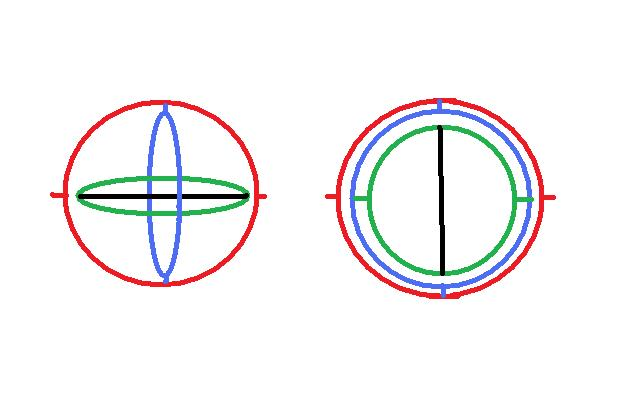
\includegraphics[width=0.9\textwidth]{images/gimbalLock.jpg}
    \label{fig:gimbal+lock}
    \caption{Kardansche Aufhängung und Gimbal lock}
\end{figure}

\begin{Bemerkung}
Man kann bei der Produktzerlegung auch andere elementare Drehmatratzen (elementare Drehachsen)  wählen, wobei
eine spezielle Wahl  zu den in der Luft und Raumfahrt verwendeten "Roll, Nick, Gier" Winkeln führen.
\end{Bemerkung}

\begin{figure}[H]
    \centering
    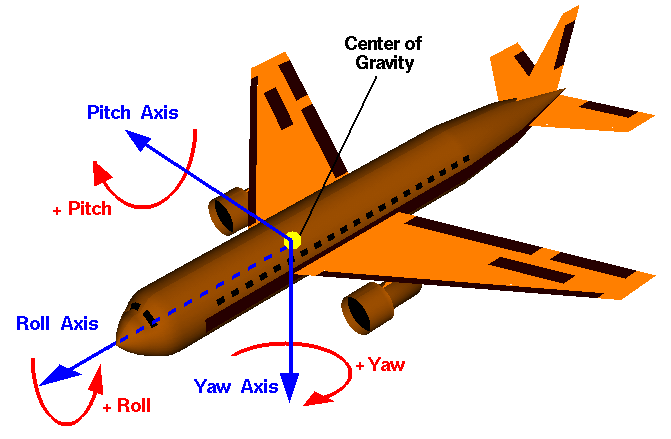
\includegraphics[width=0.9\textwidth]{images/pitch.png}
    \label{fig:roll-pitch-yaw}
    \caption{Roll, Nick und Gier Winkel}
\end{figure}

\subsection{Affiner Raum und affine Abbildungen}
Der Affine Raum $\mathbb{A}^n$ ist ein Tupel
\begin{align*}
\bigl( \mathbb{R}^n, (\mathbb{R}^n, + , \cdot ) \bigr )
\end{align*}
zusammen mit den Abbildung 
\begin{align*}
\text{---} : \mathbb{R}^n \times \mathbb{R}^n  & \to (\mathbb{R}^n, + , \cdot ) \\
\overline{PQ} & := Q-P  
\end{align*}
und
\begin{align*}
+ : \mathbb{R}^n \times (\mathbb{R}^n, + , \cdot )   & \to  \mathbb{R}^n\\
\begin{pmatrix}
P_1 \\ \vdots \\ P_n
\end{pmatrix} + \begin{pmatrix}
v_1 \\ \vdots \\ v_n
\end{pmatrix} & := \begin{pmatrix}
P_1  + v_1 \\ \vdots \\ P_n + v_n 
\end{pmatrix}   \;.
\end{align*}
Die Elemente (Vektoren) aus $\mathbb{R}^n$ nennt man auch  Punkte in Abgrenzung zu den Vektoren aus $(\mathbb{R}^n, + , \cdot )$.  
Für Punkte $P,Q \in \mathbb{R}^n$ ist also $\overline{PQ}$ ein Vektor, auch Verbindungsvektor genannt.

\begin{Definition}
Ist $B:= \{b_1, \hdots , b_n \}$ eine Basis des Vektorraums  $(\mathbb{R}^n, + , \cdot )$ und $P \in \mathbb{A}$ ein Punkt, so nennen wir das Tupel
$(P, B)$ eine affine Basis. Für jeden Punkt $Q$ gibt es dann also Skalare $\lambda_1,\hdots ,\lambda_n$ mit 
\begin{align*}
Q = P + \sum_{i=1}^{n} \lambda_i \cdot b_i  \; .
\end{align*}
Der Punkt $\begin{pmatrix}  \lambda_1 \\  \vdots \\  \lambda_n \end{pmatrix}$ heißt die Darstellung von $Q$ bezüglich der affinen Basis $(P,B)$. 
\end{Definition}



\begin{Definition}
Abbildungen der Form
\begin{align*}
\phi &: \mathbb{A} \to \mathbb{A} \\
\phi(P) & := A \cdot P + t
\end{align*} 
mit $A \in M^{n \times n}$ und $t \in (\mathbb{R}^n, + , \cdot )$ heißen affine Abbildungen.
Insbesondere heißt eine affine Abbildung mit $A = I_n$ und $t \neq 0$ Translation.
\end{Definition}

\begin{Bemerkung}
Eine Affine Abbildung
\begin{align*}
\phi &: \mathbb{A}^n \to \mathbb{A}^n \\
\phi(P) & := A \cdot P + t
\end{align*} 
ist genau dann invertierter, falls $\det(A) \neq 0$ ist und die Inverse Abbildung ist dann
\begin{align*}
\phi^{-1} &: \mathbb{A} \to \mathbb{A} \\
\phi^{-1}(P) & := A^{-1} \cdot P - A^{-1} \cdot t \; .
\end{align*} 
\end{Bemerkung}


\begin{Definition}
Sind $(P,B:= \{b_1, \hdots , b_n \})$  und $(P',B':= \{b'_1, \hdots , b'_n \})$ zwei affine Basen  und definieren wir 
die Abbildung
\begin{align*}
\theta_{(P,B)} & :  \mathbb{A}^n \to \mathbb{A}^n \\
\theta_{(P,B)}(Q) & := M_B \cdot Q - M_B \cdot P \; ,
\end{align*}
so erhalten wir analog zu der Situation in Vektorräumen
\begin{align*}
\xymatrix{
\mathbb{A}^n  \ar[d]^{\text{id}} &  & \ar[ll]^{\theta_{(P,B)}^{-1}} \mathbb{A}^n \ar[d]^{\theta_{(P,B)}^{(P',B')}} \\
\mathbb{A}^n  \ar[rr]^{\theta_{(P',B')}} & &  \mathbb{A}^n
}
\end{align*}
mit $\theta_{(P,B)}^{(P',B')} (Q) :=   \theta_{(P',B')} \biggl ( \theta_{(P,B)}^{-1} (Q) \biggr)$.
\end{Definition}


\begin{Definition}
Der Abstand von  $P,Q \in \mathbb{A}$  ist definiert durch
\begin{align*}
d : \mathbb{A} \times \mathbb{A} \to \mathbb{R} \\
d(P,Q) := || \overline{PQ} || \; .
\end{align*}
\end{Definition}


\subsubsection{Homogene Koordinaten und Projektionen}

\begin{Definition}
Der projektive  Raum ist definiert als
\begin{align*}
\mathbb{P}^n := \mathbb{R}^{n+1} / \sim \\
v \sim w \Leftrightarrow v = \lambda w \text{ für ein } \lambda \neq 0 \in \mathbb{R} \; . 
\end{align*}
\end{Definition}

Wir haben die Abbildung
\begin{align*}
\mathbb{A}^n & \to \mathbb{P}^n \\
\begin{pmatrix} p_1 \\ p_2 \\ \vdots \\ p_n \end{pmatrix} & \mapsto \begin{pmatrix} p_1 \\ p_2 \\ \vdots \\ p_n  \\  1\end{pmatrix} 
\end{align*}
und nennen das Bild eines Punktes unter dieser Abbildung die homogenen Koordinaten.
Auf der Menge der homogenen Koordinaten haben wir die Umkehrabbildung
\begin{align*}
& \mathbb{P}^n - \Biggl \{ \begin{pmatrix} p_1 \\ p_2 \\ \vdots \\ p_n  \\  p_{n+1} \end{pmatrix} \Bigg | \; p_{n+1} \neq 0 \Biggr \}   \to \mathbb{A}^n \\
& \begin{pmatrix} p_1 \\ p_2 \\ \vdots \\ p_n  \\  p_{n+1} \end{pmatrix}   \mapsto \begin{pmatrix}  \frac{p_1}{ p_{n+1}} \\ \frac{p_2}{ p_{n+1}}  \\ \vdots \\ \frac{p_n}{ p_{n+1}}  \end{pmatrix}  \; .
\end{align*}


Die Matrizenmultiplikation
\begin{align*}
\mathbb{R}^{n+1} \to \mathbb{R}^{n+1} \\
v \mapsto A \cdot v
\end{align*}
setzt sich wegen der Eigenschaft $A \cdot (\lambda v) = \lambda A \cdot v$ zu einer Abbildung
\begin{align*}
\mathbb{P}^{n} \to \mathbb{P}^{n} \\
p \mapsto A \cdot p
\end{align*}
fort. Wir können damit und mit der Definition der Matrix-Vektor-Multiplikation eine affine Abbildung 
\begin{align*}
\phi : \mathbb{R}^{n} \to \mathbb{R}^{n} \\
\phi(v):=  A \cdot v + t
\end{align*}
in homogenen Koordinate ausdrücken durch eine Matrizenmultiplikation
\begin{align*}
\begin{pmatrix} v \\ 1\end{pmatrix} \mapsto \begin{pmatrix}  A  & t  \\ 0 &1\end{pmatrix} \cdot  \begin{pmatrix} v \\ 1\end{pmatrix}   \; .
\end{align*}

\begin{Definition}
Die Abbildung 
\begin{align*}
persp_{xy} : \mathbb{A}^3 \to \mathbb{A}^2 \\
\begin{pmatrix}  X \\ Y \\ Z\end{pmatrix}  \mapsto \begin{pmatrix}  \frac{X}{\frac{Z}{d} +1 } \\   \frac{X}{\frac{Z}{d} +1 } \end{pmatrix}
\end{align*}
die Zentralprojektion auf die $X-Y$-Ebene mit Augendistanz $d$.
\end{Definition} 

\begin{Bemerkung}
Die Zentralprojektion auf die $X-Y$-Ebene mit Augendistanz $d$ lässt sich nicht durchMultiplikation mit einer  $2 \times 3$-Matrix realisieren.
\end{Bemerkung}



Definieren wir die Matrix 
\begin{align*}
K_{persp_{xy}} := \begin{pmatrix}  
1   &  0 & 0 & 0  \\
0   &  1 & 0 & 0  \\
0   &  0 & 1 & 0  \\
0   &  0 & \frac{1}{d} & 1  
\end{pmatrix} 
\end{align*}
und 
\begin{align*}
K_{orth_{xy}} := \begin{pmatrix}  
1   &  0 & 0 & 0  \\
0   &  1 & 0 & 0  \\
0   &  0 & 0 & 1  
\end{pmatrix} \; ,
\end{align*}


so können wir die Zentralprojektion auf die $X-Y$-Ebene mit Augendistanz $d$ durch die Hintereinanderausführung folgender Abbildungen darstellen:
\begin{align*}
& persp_{xy} :\mathbb{R}^3   \to \mathbb{A}^3    \to  \mathbb{A}^3    \to \mathbb{A}^2    \to \mathbb{R}^2  \\
&\begin{pmatrix} x \\ y \\ z \end{pmatrix} \mapsto \begin{pmatrix} x \\ y \\ z \\ 1 \end{pmatrix}   \mapsto K_{persp_{xy}} \cdot  \begin{pmatrix} x \\ y \\ z \\ 1 \end{pmatrix} =   \begin{pmatrix} x \\ y \\ z \\ \frac{z}{d} + 1 \end{pmatrix} \\
 & \mapsto K_{orth_{xy}} \cdot   \begin{pmatrix} x \\ y \\ z \\ \frac{z}{d} + 1 \end{pmatrix}=   \begin{pmatrix} x \\ y \\ \frac{z}{d} + 1 \end{pmatrix}   \mapsto 
 \begin{pmatrix}  \frac{x}{\frac{z}{d} +1 } \\   \frac{x}{\frac{z}{d} +1 } \end{pmatrix}
 \end{align*}
\section{Kurven, Flächen und  Netze}
Die rechnergestützte Beschreibung von Kurven und Flächen ist ein wichtiges Gebiet der Computergrafik.
Es ermöglicht die Berechnung geometrischer und physikalischer  Eigenschaften von Körpern so wie deren graphische Darstellung.
Eine zentrale Rolle spielen hierbei geometrische Objekte, die durch Punkte, Kanten und einfache Flächen, wie zum Beispiel Dreiecke oder Vierecke, beschrieben werden können. Man spricht dann auch entsprechend von Dreicks- bzw. Vierecksnetzen. Häufig sind dabei nicht alle möglichen Konstruktionen zulässig und es hat sich ein Struktur herausgebildet, die für die Computergrafik besonders geeignet ist. Zum einen, weil seine grafische Darstellung besonders schnell und einfach möglich ist und zum anderen, weil viele Berechnungen bestimmte Voraussetzungen benötigen, man denke da zum Beispiel an die Oberfläche oder das Volumen eines Körpers.
Von Bedeutung sind in diesem Kontext auch geeignete Datenstrukturen, mit deren Hilfe sich diese Strukturen und gängige Berechnungen effizient verarbeiten lassen. 
Ein weiterer wichtiger Aspekt ist das generieren und modellieren solcher Strukturen. Hierbei treten häufig sogenannte Interpolationsprobleme auf. Sie entstehen aus dem Wunsch heraus, Kurven und Flächen nur durch die Angabe von Punkten zu generieren. 

\subsection{Polygone, Netze und Elemente der diskreten Geometrie}
\begin{Definition}
Ein geschlossenes Polygon ist ein Paar $P:=(V_P,E_P)$, wobei   
\begin{align*}
E_P := \{e_0, \hdots, e_k \} \subset \mathbb{A}^3,
\end{align*}
eine geordnete Menge von paarweise verschiedenen Punkten, die auch Ecken genannt werden, und   
\begin{align*}
K_P: = \biggl \{(e_0,e_1)  \hdots, (e_{k-1},e_k), (e_k,e_0) \biggr\} \subset \mathbb{A}^3 \times \mathbb{A}^3
\end{align*}
die zugehörige Menge der gerichteten Kanten ist. 
Ist $(e_{l-1},e_l) \in K_p$ eine gerichtete Kante, so bezeichnen wir mit 
\begin{align*}
|(e_{l-1},e_l)| := \bigl \{ e_{l-1} + t \cdot \overline{e_{l-1}e_{l}} \; \big  | \; t \in [0,1] \bigr \} 
\end{align*}
ihre geometrische Realisierung oder einfach Kante und mit 
\begin{align*}
|P|:= \bigcup_{(e_{l-1},e_l) \in K_P} |(e_{l-1},e_l)|
\end{align*}
 die geometrische Realisierung des Polygons oder geometrisches Polygon.


Ein (geschlossenes) Polygon heißt \textbf{einfach}, falls der Schnitt zweier geometrischer Kanten  entweder leer oder genau ein Punkt aus $V$ ist.
Es heißt \textbf{planar}, falls alle Punkte $e \in V_P$ in einer Ebene liegen.
\end{Definition}


\begin{figure}[H]
    \centering
    \input{images/xfig/polygon_closed.pdf_t}
    \caption{Geschlossenes Polygon}
    \label{fig:polygon-closed}
\end{figure}

\begin{Definition}
Wir nennen  ein geschlossenes Polygon $P'$ eine \textbf{Nummerrierung} von $P$, falls 
$E_{P'} =E_{P}$ (als Mengen) und
$|P'| = |P|$ ist. 
\end{Definition}


Wie wir gleich sehen werden, definiert die Reihenfolge der Punkte eines einfachen, geschlossenen, planaren Polygons eine Orientierung. Um diesen Sachverhalt präzise definieren zu können, benötigen wir einen Satz, der 
auf den ersten Blick als selbstverständlich erscheint aber rein mathematisch betrachtet tatsächlich schwer zu beweisen ist. Es handelt sich um den Jordanschen Kurvensatz:

\begin{Satz}
Sei $P$ ein einfaches, geschlossenes, planares Polygon und $U$ die Ebene, in der alle seine Punkte liegen. 
Dann unterteilt die geometrische Realisierung $|P|$ die Ebene $U$ in genau zwei Gebiete, ein beschränktes, das das Innere des Polygons genannt wird, und ein unbeschränkte, das das Äußere des Polygons genannt wird.
\end{Satz}

\begin{Definition}
Wir bezeichnen das Innere eines Polygons $P$ mit $|\overset{\circ}{P}|$.
\end{Definition}

Mit Hilfe des Jordanschen Kurvensatzes können wir nun sagen, was die Durchlaufrichtung einer Kante ist und schließlich ob ein Polygon mit oder gegen den Uhrzeigersinn orientiert ist.

\begin{Definition}
Sei $P$ ein einfaches, geschlossenes, planares Polygon. Eine gerichtete Kante $(e_{l-1}, e_l) \in E_P$ hat \textbf{positive Durchlaufrichtung}, falls beim Durchlaufen der  Kante $|(e_{l-1}, e_l)|$ von $e_{l-1}$ nach $e_l$ das innere des Polygons stets rechts von der Kante liegt und \textbf{negative Durchlaufrichtung}, falls es stets links von ihr liegt. 
\end{Definition} 
 
\begin{Definition}
Ein einfaches, geschlossenes, planares Polygon $P$ heißt im Uhrzeigersinn orientiert, falls eine und damit alle gerichteten Kanten positive Durchlaufrichtung haben und entsprechend gegen den Uhrzeigersinn orientiert bei negativer Durchlaufrichtung.  
\end{Definition} 

\begin{figure}[H]
    \centering
    \input{images/xfig/polygon_orientation.pdf_t} \\
    \input{images/xfig/polygon_orientation_c.pdf_t}
    \caption{Gerichtete Polygone}
    \label{fig:polygon-oriented}
\end{figure}

Netze bestehen nun im wesentlichen aus an den Kanten zusammengeklebten, einfachen, geschlossenen, planaren Polygonen.

\begin{Definition}
Sei $N:= \bigcup P_i$ die Vereinigung endlich vieler, einfacher, geschlossener, planarer Polygone, 
$E_N := \bigcup E_{P_i}$ und $K_N := \bigcup E_{P_i}$ die Vereinigung der Ecken beziehungsweise der Kantenmengen.
Analog zu der Definition eines Polygons definieren wir die geometrischen Realisierungen 
$|K_N| := \bigcup |P_i|$ und $|N| := \bigcup |\overset{\circ}{P_i}| \bigcup |K_N|$
\begin{itemize}
\item Dann heißt $N$ \textbf{Netz}, falls Der Schnitt zweier Polygone entweder leer, ein Punkt in $E_N$ oder eine Kante in $K_N$ ist. 

\item Die Menge aller Kanten, die nur zu einem Polygon gehören, heißt Rand von $N$ und wird mit $\partial N$ bezeichnet.
\item Ein Netz heißt \textbf{geschlossen}, falls es keinen Rand gibt, in Zeichen $\partial N = \emptyset$. 
\item Die Polygone des Netzes werden auch als Facetten bezeichnet.
\end{itemize}
\end{Definition} 


Durch die  Orientierung von Polygonen können wir nun den Begriff der Orientierung und der Orientierbarkeit eines Netzes einführen.

\begin{Definition}
Ein Netz $N$ heißt orientierbar, falls man alle seine Polygone so nummerieren kann, dass jede gemeinsame Kante zweier Polygone jeweils entgegengesetzt gerichtet ist. 
\end{Definition}


\begin{figure}[H]
    \centering
    \input{images/xfig/surface_orientable.pdf_t}
    \caption{Orientierbare Fläche}
    \label{fig:surface-orientable}
\end{figure}

\begin{Bemerkung}
Ist eine Fläche orientierbar und nummeriert man die Polygone so, dass benachbarte Kanten entsprechend der Definition immer entgegengesetzt gerichtet sind, so sind entweder alle seine Polygone im oder alle seine Polygone gegen den Uhrzeigersinn orientiert.
\end{Bemerkung}

\begin{figure}[H]
    \centering
    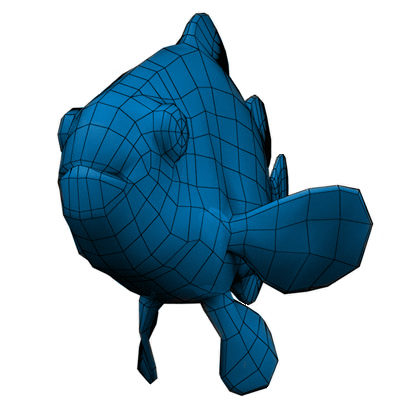
\includegraphics[width=0.4\textwidth]{images/clown_fish.jpg}
    \caption{Ein geschlossenes, orientierbares Netz. Quelle:CGAL}
    \label{fig:closed-orientable-mesh}
\end{figure}

\begin{figure}[H]
    \centering
    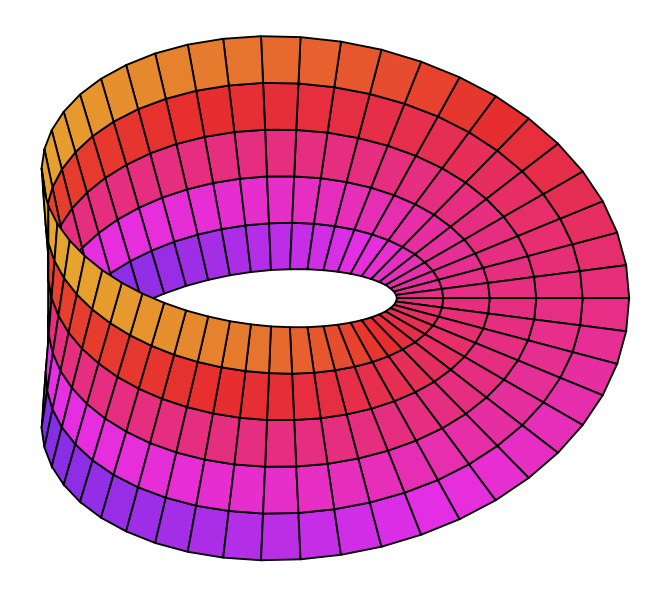
\includegraphics[width=0.4\textwidth]{images/Moebius_strip.png}
    \caption[Möbiusband. Quelle:Wikipedia]
             {Das sogenannte Möbiusband ist hingegen nicht orientierbar. 
             Es ist nicht geschlossen, sondern hat einen zusammenhängenden Rand. 
             Quelle:Wikipedia}
    \label{fig:moebius-strip}
\end{figure}

\begin{Definition}
Eine Orientierung ist die Wahl einer Klasse von Nummerierungen, so dass alle Polygone entweder im oder gegen den Uhrzeigersinn orientiert sind.
\end{Definition}

\begin{Bemerkung}
Ein Netz hat entweder genau zwei oder keine Orientierung.  
\end{Bemerkung}


\begin{Definition}
Sei $N$ ein orientierbares Netz mit einer Orientierung so gewählt, dass  alle Polygone gegen den Uhrzeigersinn orientiert sind. Wählt man für jedes Polygon $P_i \in N$ drei benachbarte Ecken $e_{j-1}^{P_i}, e_{j}^{P_i}$ und $e_{j+1}^{P_i}$, so erhalten wir
mit $n_{P_i} = e_{j}^{P_i}e_{j+1}^{P_i} \times e_{j}^{P_i}e_{j-1}^{P_i}$ einen Vektor, der Senkrecht auf der Ebene steht in der das Polygon liegt. Wir nennen die Menge $\{P_0, \hdots, P_n\}$ das äußere Normalenfeld des Netzes. 
\end{Definition}


\begin{figure}[H]
    \centering
    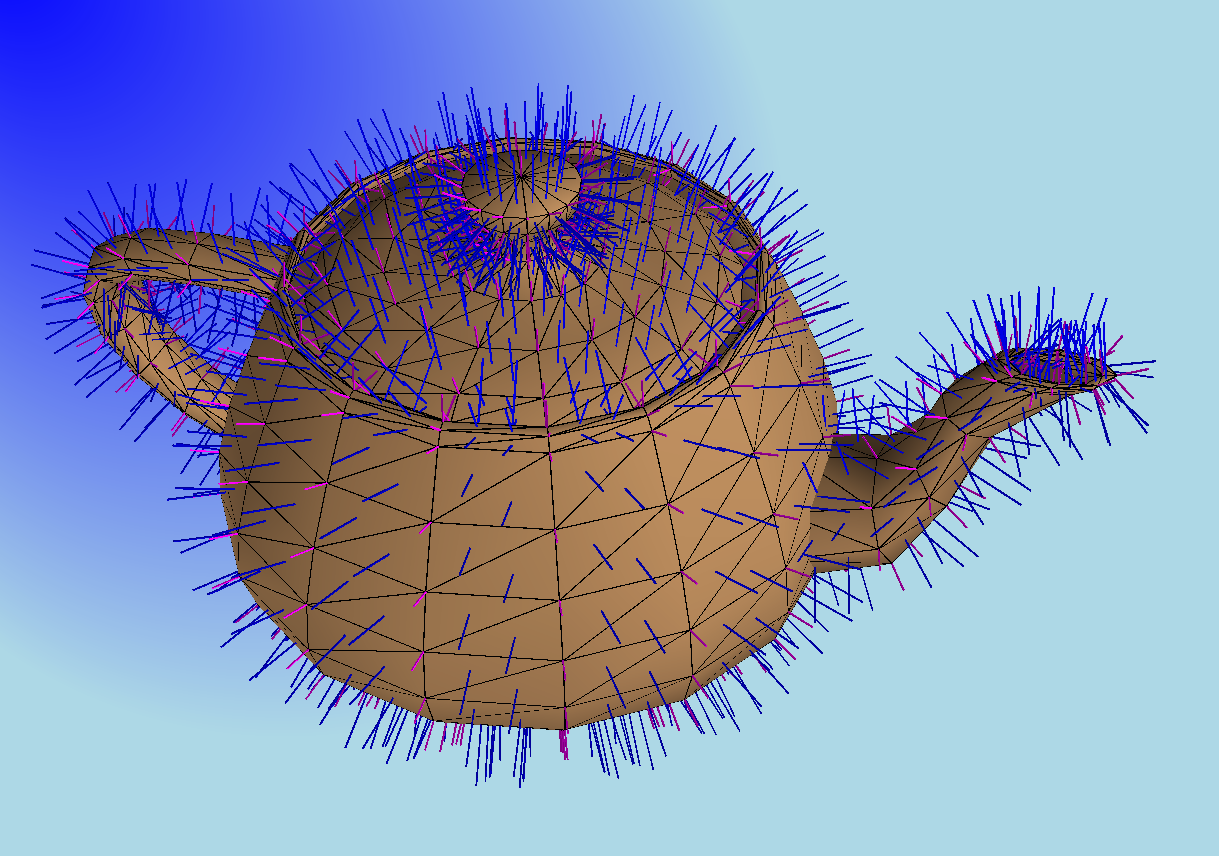
\includegraphics[width=0.7\textwidth]{images/teapot-normals.png}
    \caption{Das äußere Normalenfeld}
    \label{fig:outer-normals}
\end{figure}
Eine wichtige Größe für ein Netz ist die sogenannte Eulercharakteristik, welche in direkter Beziehung zum sogenannten Geschlecht eines Netzes steht.

\begin{Definition}
$N:= \bigcup P_i$ ein Netz. Dann ist die Eulercharacteristig definiert als
\begin{align*}
\chi(N):= \#(E_N) - \#(|K_N|) + \#(N) 
\end{align*}
Sie ist also die Anzahl der  Punkte, minus die Anzahl der geometrischen Kanten, plus die Anzahl der Facetten.
\end{Definition}

Das Geschlecht eines geschlossenen Netzes ist anschaulich gesprochen die Anzahl an Löchern, die durch das geometrische Netz hindurch gehen. Dies lässt sich mit einigem Aufwand mathematisch präzise definieren, jedoch für unsere Zwecke reicht eine Definition durch Beispiele.
\begin{Definition}
Sei $N$ ein geschlossenes Netz. Dann bezeichnen wir mit
\begin{align*}
g(N):= \textbf{Anzahl der Löcher in } |N|
\end{align*}
\end{Definition}
Beispiele:

\begin{figure}[H]
    \centering
    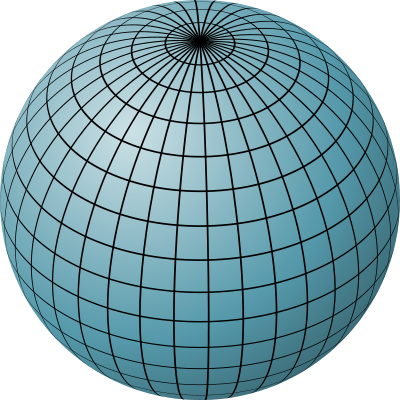
\includegraphics[scale=0.2]{images/Sphere.png}
    \caption{Geschlossenes Netz vom Geschlecht $0$. Quelle:Wikipedia}
    \label{fig:closed-mesh-gender0}
\end{figure}


\begin{figure}[H]
    \centering
    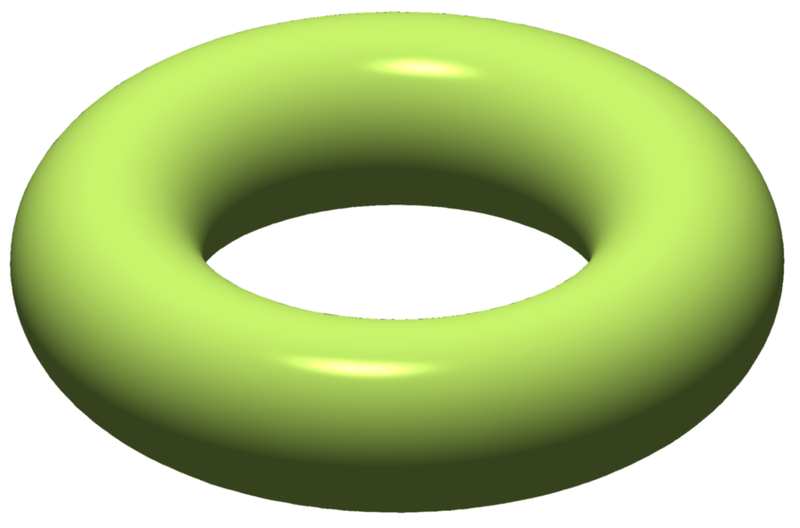
\includegraphics[scale=0.8]{images/Torus.png}
    \caption{Geschlossenes Netz vom Geschlecht $1$. Quelle:Wikipedia}
    \label{fig:closed-mesh-gender1}
\end{figure}


\begin{figure}[H]
    \centering
    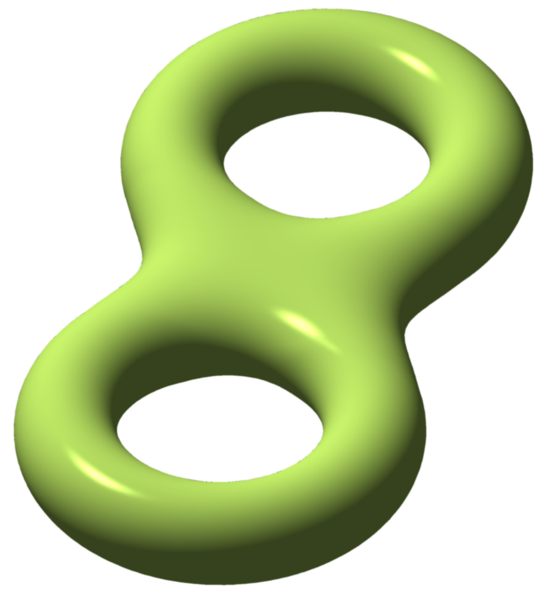
\includegraphics[scale=1.0]{images/Double_torus.png}
    \caption{Geschlossenes Netz vom Geschlecht $2$. Quelle:Wikipedia}
    \label{fig:closed-mesh-gender2}
\end{figure}

\begin{figure}[H]
    \centering
    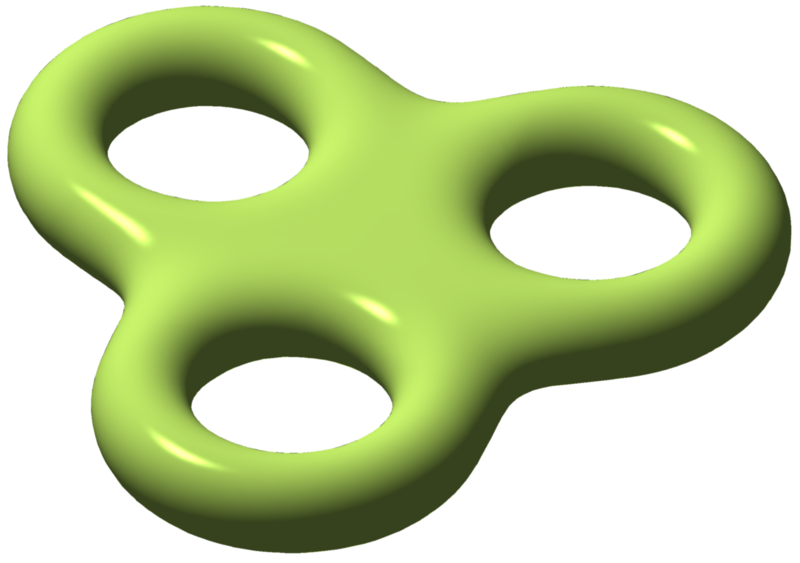
\includegraphics[scale=1.0]{images/Triple_torus.png}
    \caption{Geschlossenes Netz vom Geschlecht $3$. Quelle:Wikipedia}
    \label{fig:closed-mesh-gender3}
\end{figure}

Der Zusammenhang zwischen der Eulercharacteristik und dem Geschlecht wurde im allgemeinen Fall von dem Mathematiker  
Henri Poincare und vorher in einem Spezialfall von Leonard Euler bewiesen. 
\begin{Satz}
Für ein geschlossenes Netz $N$ gilt $\chi(N) = 2 - 2g(N)$. 
\end{Satz}

\begin{Bemerkung}
Nach dem Satz lässt sich das Geschlecht und somit die Anzahl der Löcher via $g(N) = \frac{2- \chi(N)}{2}$ berechnen.
\end{Bemerkung}

\subsection{Datenstrukturen}
\begin{Definition}
Eine Liste ist eine Datenstruktur, in der man Objekte unter Beachtung der 
Reihenfolge speichern kann. 
Für eine Liste von Objekten $O_1,~\hdots,~O_n$ verwenden wir die Notation 
\begin{equation*}
    E = (O_1,~\hdots,~O_n )
\end{equation*}
Jedes Element kennt seinen Vorgänger und Nachfolger und man kann direkt 
auf das $i$-te Element zugreifen:
\begin{equation*}
    %TODO: maybe nicer placement possible here?
    \begin{matrix}
        E[i] & := & O_i \\
        \textrm{prev}(E[i]) & := & O_{i-1} \\
        \textrm{next}(E[i]) & := & O_{i+1} \\
    \end{matrix}
\end{equation*}
Dabei bezeichnet $\textrm{prev}(E[i])$ den Vorgänger und $\textrm{next}(E[i])$ 
den Nachfolger, wobei 
\begin{equation*}
    \forall l \in \mathbb{N} : \{E[l] = \textrm{NULL}~|~(l>n) \vee (l<0)\}
\end{equation*}
$i$ wird auch als Index des $i$-ten Listenelements bezeichnet. 
\end{Definition}

\begin{Definition}[Eckenliste]

In einer Liste $E = (e_1, e_2, \hdots, e_n)$ werden Referenzen auf die Ecken 
gespeichert. 
Eine Referenz im $\mathbb{R}^3$ könnte so aussehen: 
\begin{equation*}
    e_k = \begin{pmatrix}
        x_k \\
        y_k \\
        z_k
    \end{pmatrix}
\end{equation*}
Die $i$-te Facette wird als Liste $F_i = \bigl( i_1,~\hdots,~i_l  \bigr)$ von 
Referenzen auf die Eckenliste gespeichert. 
Die $k$-te Ecke der $i$-ten Facette kann so z.B. mit $E[F_i[k]]$ referenziert 
werden. 
\end{Definition}
\begin{multicols}{2}[Vor- und Nachteile:]
    \begin{itemize}
        \item[+] Einfach zu implementieren
        \item[+] Orientierung kann durch Konvention gespeichert werden
        \vspace{60pt}
        \item[-] Nachbarschaftsbeziehungen nicht enthalten / schwierig zu 
                 berechnen
        \item[-] Die Zugehörigkeit einer Ecke zu einer Kante muss immer 
                 berechnet werden
        \item[-] Point-in-Mesh, Abstandsberechnungen,  Schnittprobleme und ähnliches fast unmöglich zu berechnen
    \end{itemize}
\end{multicols}

\begin{Definition}[Kantenliste]

In einer Liste $E = (e_1,~e_2,~\hdots,~e_n)$ werden Referenzen auf die Ecken 
gespeichert. 
In einer Liste $K$ werden die Kanten  in einer zwei Elementen Liste von Indizes auf die Eckenliste 
abgespeichert: 
\begin{equation*}
    K = \bigl( (i_{e_1},i_{e_n}),~\hdots,~
               (i_{e_1},i_{e_m}) \bigr)
\end{equation*}
Die $k$-te Facette wird als Liste von Indizes auf die Kantenliste 
gespeichert: 
\begin{equation*}
    F_k = \bigl( j_1,\hdots,j_l \bigr)
\end{equation*}
In einer Liste $M$ werden die Indizes auf Facetten in einer zwei Elementen Liste abgespeichert, 
die die entsprechende Kante in der Kantenliste als Kante haben: 
\begin{equation*}
    M = \bigl( (i_1,i_2),~\hdots,~(l_1,l_2) \bigr )
\end{equation*}
$M[i] \in M$ sind also zwei Facetten, die $K[i] \in K$ als Kante haben. 
Der erste Eintrag der Facette befindet sich links und der zweite rechts von der 
Kante. 
Ist die Kante eine Randkante, so wird der andere Wert auf $-1$ 
gesetzt. 



\end{Definition}
\begin{multicols}{2}[Vor- und Nachteile:]
    \begin{itemize}
        \item[+] Nachbarschaftsbeziehungen der Polygone werden gespeichert 
        \item[-] Orientierung der Kanten geht verloren (schwierig zu speichern) 
    \end{itemize}
\end{multicols}

\begin{Definition}[Halfedge]

In einer Liste $E = (e_1,~e_2,~\hdots,~e_n)$ werden Referenzen auf die Ecken 
gespeichert. 
Es wird eine Datenstruktur namens Halfedge eingeführt. 
Eine Halfedge $e$ besitzt\footnote{Siehe auch Abbildung \vref{fig:halfedge}}: 
\begin{itemize}
    \item Indizex auf den Anfangs- und Endpunkt ($i_b$ und $i_e$)
    \item Referenzen auf die gegenüberliegende Kante $\textrm{twin}(e)$\\
          (Bei dieser sind die Anfangs- und Endpunkte vertauscht.)
    \item Referenzen auf die vorangehende $\textrm{prev}(e)$ und die folgende 
          $\textrm{next}(e)$ Halfedge
    \item Referenz auf die Facette, die sie berandet
\end{itemize}
Die unendliche oder äußere Zelle wird wieder mit $-1$ bezeichnet. 
Eine Facette ist dann eine Liste mit Referenzen von Halfedges, beziehungsweise 
reicht auch die Referenz auf eine Halfedge.

\end{Definition}
\begin{multicols}{2}[Vor- und Nachteile:]
    \begin{itemize}
        \item[+] Alle kombinatorischen Daten werden effizient gespeichert
        \item[+] Auch die Orientierung der Kanten bleibt erhalten
        \vspace{10pt}
        \item[-] Die Implementierung ist komplex
        \item[-] Overhead durch große Datenmengen
        \item[-] Nur für orientierbare Netze nutzbar
    \end{itemize}
\end{multicols}

\begin{figure}[H]
    \centering 
    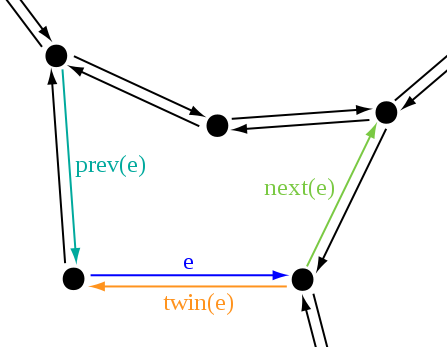
\includegraphics[scale=0.5]{images/halfedge.png}
    \caption{Halfedge. Quelle:Wikipedia}
    \label{fig:halfedge}
\end{figure}

\subsubsection{Subdivision}



\subsection{Modellierung}

\subsubsection{Parameterdarstellungen}

\begin{Definition}
Eine Kurve ist eine  Abbildung 
\begin{align*}
c: I \subset \mathbb{R} \to \mathbb{R}^3 \\
c(t) := \begin{pmatrix} x(t) \\  y(t) \\ z(t) \end{pmatrix}
\end{align*}
bei der die Funktionen $x, y, z : I \to \mathbb{R}$ stetig sind. Sie heisst differenzierbar, falls $x,y,z$ differenzierbar sind und die Ableitung ist dann definiert als 
\begin{align*}
c': I \subset \mathbb{R} \to \mathbb{R}^3 \\
c'(t) := \begin{pmatrix} x'(t) \\  y'(t) \\ z'(t) \end{pmatrix} \; .
\end{align*}
 \end{Definition}

\begin{Beispiel}
Die Kurve 
$c : [0, 2\pi]  \to  \mathbb{R}^3$, $c(t) :=  \begin{pmatrix} r \cos(t) \\ r  \sin(t) \\  0 \end{pmatrix}$
beschreibt einen Kreis mit Radius $r$, der in der XY-Ebene liegt. Die Ableitung ist
\begin{align*}
c'(t) =  \begin{pmatrix} (r \cos(t))' \\  (r\sin(t))' \\  0 \end{pmatrix} = \begin{pmatrix} -r \sin(t) \\ r \cos(t) \\  0 \end{pmatrix} \;.
\end{align*} 
\end{Beispiel}

\begin{Beispiel}
Die Kurve 
$c :  \mathbb{R}   \to  \mathbb{R}^3$, $c(t) :=  \begin{pmatrix} \cos(t) \\  \sin(t) \\  t \end{pmatrix}$
beschreibt eine sogenannte Helix. Die Ableitung ist
\begin{align*}
c'(t) =  \begin{pmatrix} \cos'(t) \\  \sin'(t) \\  t'  \end{pmatrix} = \begin{pmatrix} -\sin(t) \\  \cos(t) \\  1 \end{pmatrix} \;.
\end{align*} 
\end{Beispiel}
\begin{figure}[H]
    \centering
    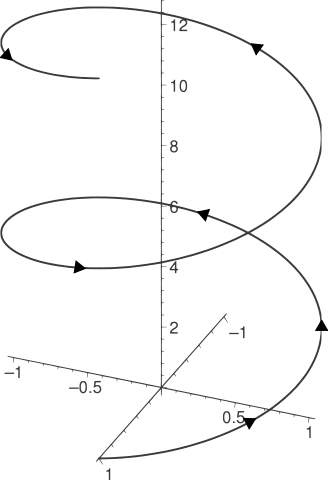
\includegraphics[scale=0.45]{images/Helix.png}
    \caption{Eine Helix. Quelle:Wikipedia}
    \label{fig:helix}
\end{figure}

\begin{Definition}
Ist $c: I \subset \mathbb{R} \to \mathbb{R}^3$ eine stückweise differenzierbare Kurve, so heißt
\begin{align*}
l(c) := \int_{I} ||c'(t)|| dt
\end{align*}
ihre Länge.
\end{Definition}


\begin{Definition}
Ein Fläche ist   eine Abbildung
\begin{align*}
s: U \subset \mathbb{R}^2 \to \mathbb{R}^3 \\
s(u,v) := \begin{pmatrix} x(u,v) \\ y(u,v) \\ z(u,v) \end{pmatrix} 
\end{align*} 
bei der die Abbildungen $x, y, z : U \subset \mathbb{R}^2 \to \mathbb{R}^3$ stetig sind. Sie heißt differenzierbar, falls die partiellen Ableitungen
\begin{align*}
\frac{\partial}{\partial u} s(u,v) = \begin{pmatrix}  \frac{\partial}{\partial u} x(u,v) \\  \frac{\partial}{\partial u} y(u,v) \\  \frac{\partial}{\partial u} z(u,v) \end{pmatrix}
\end{align*}
und 
\begin{align*}
\frac{\partial}{\partial v} s(u,v) =  \begin{pmatrix} \frac{\partial}{\partial v} x(u,v) \\ \frac{\partial}{\partial v} y(u,v) \\ \frac{\partial}{\partial v} z(u,v) \end{pmatrix}
\end{align*}
existieren. Die Ebene 
\begin{align*}
T_s(u,v) :=  \{ s(u,v) + \lambda \cdot \frac{\partial}{\partial u} s(u,v) + \mu \cdot \frac{\partial}{\partial v} \; | \; \lambda, \mu \in \mathbb{R} \}
\end{align*}
heißt Tangentialebene am Punkt $(u,v)$ und  der Vektor 
\begin{align*}
n (u,v):= \frac{\partial}{\partial u} s(u,v) \times \frac{\partial}{\partial v} s(u,v) \; ,
\end{align*}
welcher Senkrecht auf dieser Ebene steht,  die Normale.
\end{Definition}



\subsubsection{Bezier Kurven und Flächen}
\begin{Definition}
Die Bernsteinpolynome vom Grad $n$ sind definiert als
\begin{align*}
B_i^n(t) := \begin{pmatrix} n \\ i \end{pmatrix} (1-t)^{n-i}t^i
\end{align*}
mit $i = 0, \hdots n$, $t \in [0,1]$ und dem Binomialkoeffizient
\begin{align*}
\begin{pmatrix} n \\ i \end{pmatrix} := \frac{n!}{i!(n-i)!} = \frac{n(n-1) \cdots 1}{i(i-1) \cdots 1 (n-i) (n-i-1) \cdots 1 } \; .
\end{align*}
\end{Definition}

\begin{figure}[H]
    \centering
    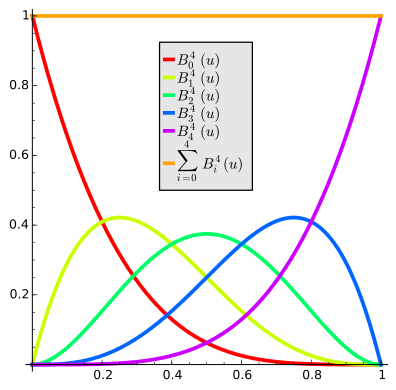
\includegraphics[scale=0.8]{images/Bernstein_Polynomials.png}
    \caption{Die Bernsteinpolynome $B^{4}_i$ und deren Summe. Quelle:Wikipedia}
    \label{fig:bernstein-polynomial}
\end{figure}

\begin{Bemerkung}
Die Bernsteinpolynome vom Grad $n$ bilden eine Basis des Vektorraums der Polynome vom Grad $n$ im Intervall $[0,1]$.
\end{Bemerkung}

\begin{Satz}
Es gilt die Rekursionsformel
\begin{align*}
B_i^n(t) = (1-t) \cdot B^{n-1}_{i}(t) + t \cdot B^{n-1}_{i-1}(t)
\end{align*}
mit $B^0_0(t) = 1$ und $B^i_n(t) = 0$ für $i<0$ oder $i>n$.
\end{Satz}
\begin{proof}
Folgt fast direkt aus der Rekursionsformel des Binomialkoeffizienten
\begin{align*}
\begin{pmatrix} n \\ i \end{pmatrix} = \begin{pmatrix} n-1 \\ i \end{pmatrix} + \begin{pmatrix} n-1 \\ i-1 \end{pmatrix} 
\end{align*}
\begin{figure}[H]
    \centering
    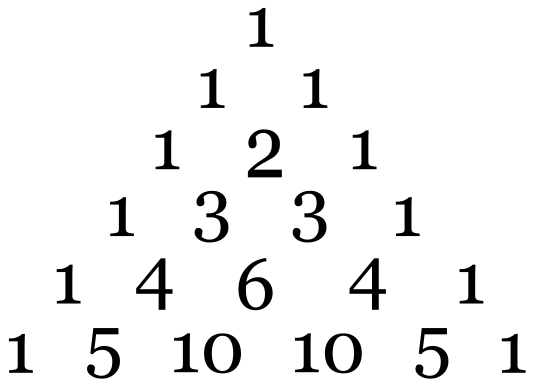
\includegraphics[scale=0.2]{images/pascal.png}
    \caption{Pascalsches Dreieck}
    \label{fig:pascals-triangle}
\end{figure}
\end{proof}


\begin{Definition}
Seien $b_0, \hdots b_n \in \mathbb{R}^3$. Dann heißt die Kurve
\begin{align*}
B^n(t) := \sum_{i = 0}^{n} B_i^n(t) \cdot  b_i \; , t \in [0,1] 
\end{align*} 
eine Bezierkurve vom Grad $n$. Die $b_i$ werden auch Kontrollpunkte genannt.
Für ein beliebiges Intervall $[a,b]$ definieren wir
\begin{align*}
B^n_{[a,b]} (t):=  B^n\biggl( \frac{t-a }{a-b} \biggr) \; , t \in [a,b] \; .
\end{align*} 
\end{Definition}


\begin{Satz}
Eine Bezierkurve hat die Ableitung
\begin{itemize}
\item $(B^n)'(t) = n \cdot \sum_{j = 0}^{n-1} B_{j}^{n-1}(t) \cdot (b_{j+1} - b_j) \; ,$ und nach der Kettenregel
\item $(B^n_{[a,b]})'(t) = \frac{1}{b-a} (B^n)' \bigl(\frac{t -a}{b-a} \bigr)$  für ein beliebiges Parameterintervall.
\end{itemize}
\end{Satz}

\begin{Satz}[Algorithmus von de Casteljau]
Sei $B^n(t) := \sum_{i = 0}^{n} B_i^n(t) \cdot  b_i$ eine Bezierkurve. Für ein 
$t_0 \in [0,1]$ definieren wir rekursiv  
\begin{align*}
b_i^k := \begin{cases}
b_i   & i= 0, \hdots,  n \\
(1-t_0) \cdot b_{i-1}^{k-1} + t_0 \cdot b_{i}^{k-1} &  i = 1, \hdots , n \; \;   k = 1, \hdots , i 
\end{cases} 
\end{align*}
was sich schematisch folgendermaßen darstellen lässt: 
\begin{align*}
\xymatrix{
b_0   \ar@{}[r]|-{=}  &  b_0^0 \ar[dr]^{\cdot(1-t_0)}  &  & & & & & &  \\
b_1   \ar@{}[r]|-{=}  &  b_1^0  \ar[r]^{\cdot t_0} \ar[dr]^{\cdot(1-t_0)} &   b_1^1  \ar[dr]^{\cdot(1-t_0)} & & & & & & \\
b_2   \ar@{}[r]|-{=}  \ar@{..}[d] &  b_2^0  \ar[r]^{\cdot t_0}  \ar@{..}[d] &   b_2^1 \ar[r]^{\cdot t_0}  \ar@{..}[d] &  b_2^2   \ar@{..}[dr]& & & & & \\
b_{n-1}   \ar@{}[r]|-{=}  &  b_{n-1}^0   \ar[r]^{\cdot t_0}  \ar[dr]^{\cdot(1-t_0)} &    b_{n-1}^1   \ar[r]^{\cdot t_0}  \ar[dr]^{\cdot(1-t_0)} &  b_{n-1}^2  \ar@{..}[r] &  
b_{n-1}^{n-1}  \ar[dr]^{\cdot(1-t_0)} & & & & \\
b_{n}   \ar@{}[r]|-{=}  &  b_{n}^0  \ar[r]^{\cdot t_0}  &    b_{n}^1   \ar[r]^{\cdot t_0}  &  b_{n}^2  \ar@{..}[r] & b_{n}^{n-1}   \ar[r]^{\cdot t_0}& b_{n}^{n}& & & 
}
\end{align*}
Dann gilt $b_n^n = B^n(t_0)$.
\end{Satz}

\begin{figure}[H]
    \centering
    \input{images/xfig/deCasteljau.pdf_t}
    \caption{} %TODO
    \label{fig:deCastel}
\end{figure}



\begin{Definition}[Patching]
Seien $B^n(t)$ und $(B^*)^m(t)$  Bezierkurven. Man spricht von einem $C^0$-Patching (an der Stelle $B^n(1)$), falls
 $B^n(1) = (B^*)^m(0) $ gilt. Stimmen auch die Ableitungen überein, also  $(B^n)'(1) = ((B^*)^m)'(0) $, dann spricht man von einem $C^1$-Patching und stimmen noch für $k> 1$ auch
die höheren Ableitungen $(B^n)^{k}(1) = ((B^*)^m){k}(0) $ überein, so spricht man von einem $C^k$-Patching . 
 \end{Definition}


\begin{figure}[H]
    \centering
    \input{images/xfig/bezier_patch.pdf_t}
    \caption{Bezier Patch}
    \label{fig:bezier-patch}
\end{figure}

\begin{Bemerkung}
Zwei Bezierkurven   $B^n(t) := \sum_{i = 0}^{n} B_i^n(t) \cdot  b_i$ und $(B^*)^m(t) := \sum_{i = 0}^{m} B_i^n(t) \cdot  b^*_i$ bilden genau dann einen $C^1$-Patch  (an der Stelle $B^n(1)$), wenn 
$B^n(1) = (B^*)^m(0)$ und $\Bigl(B^n(1) - b_{n-1} \Bigr)= - \frac{m}{n}  \Bigl((B^*)^m(0) - (b^*)_1 \Bigr)$ gilt.
\end{Bemerkung}


\begin{Definition}
Ist  $B^n(t)$ eine Bezierkurve, so bilden die Bezierkurven $(B^{*})^n(t)  :=  \sum_{i = 0}^{n} B_i^n(t/2) \cdot  b_i^i$ und  $(B^{**})^n(t)  :=  \sum_{i = 0}^{n} B_i^n(t/2) \cdot  b_n^{n-i}$
einen $C^1$-Patch.
\end{Definition}


\begin{Definition}
Ersetzt man in einer Bezierkurve 
\begin{align*}
B^m(v) := \sum_{j = 0}^{m} B_j^m(v) \cdot  b_j
\end{align*}
vom Grad $m$ die Kontrollpunkte $b_j$ durch $m+1$ Bezierkurven
\begin{align*}
b_j (u)= \sum_{i = 0}^{n} B_i^n(u) \cdot  b_{ij}
\end{align*}
 vom Grad $n$ mit jeweils $n+1$ Kontrollpunkten $ b_{ij}$ für $i = 0, \cdots , n$, so erhält man eine Fläche
\begin{align*}
F(u,v) =  \sum_{i = 0}^{n}  \sum_{j = 0}^{m} B_i^n(u) B_j^m(v) \cdot  b_{ij} \; ,
\end{align*}
welche auch Tenorprodukt-Fläche der Bezierkurven  oder einfach Bezierfläche genannt wird.
\end{Definition}


\begin{figure}[H]
    \centering
    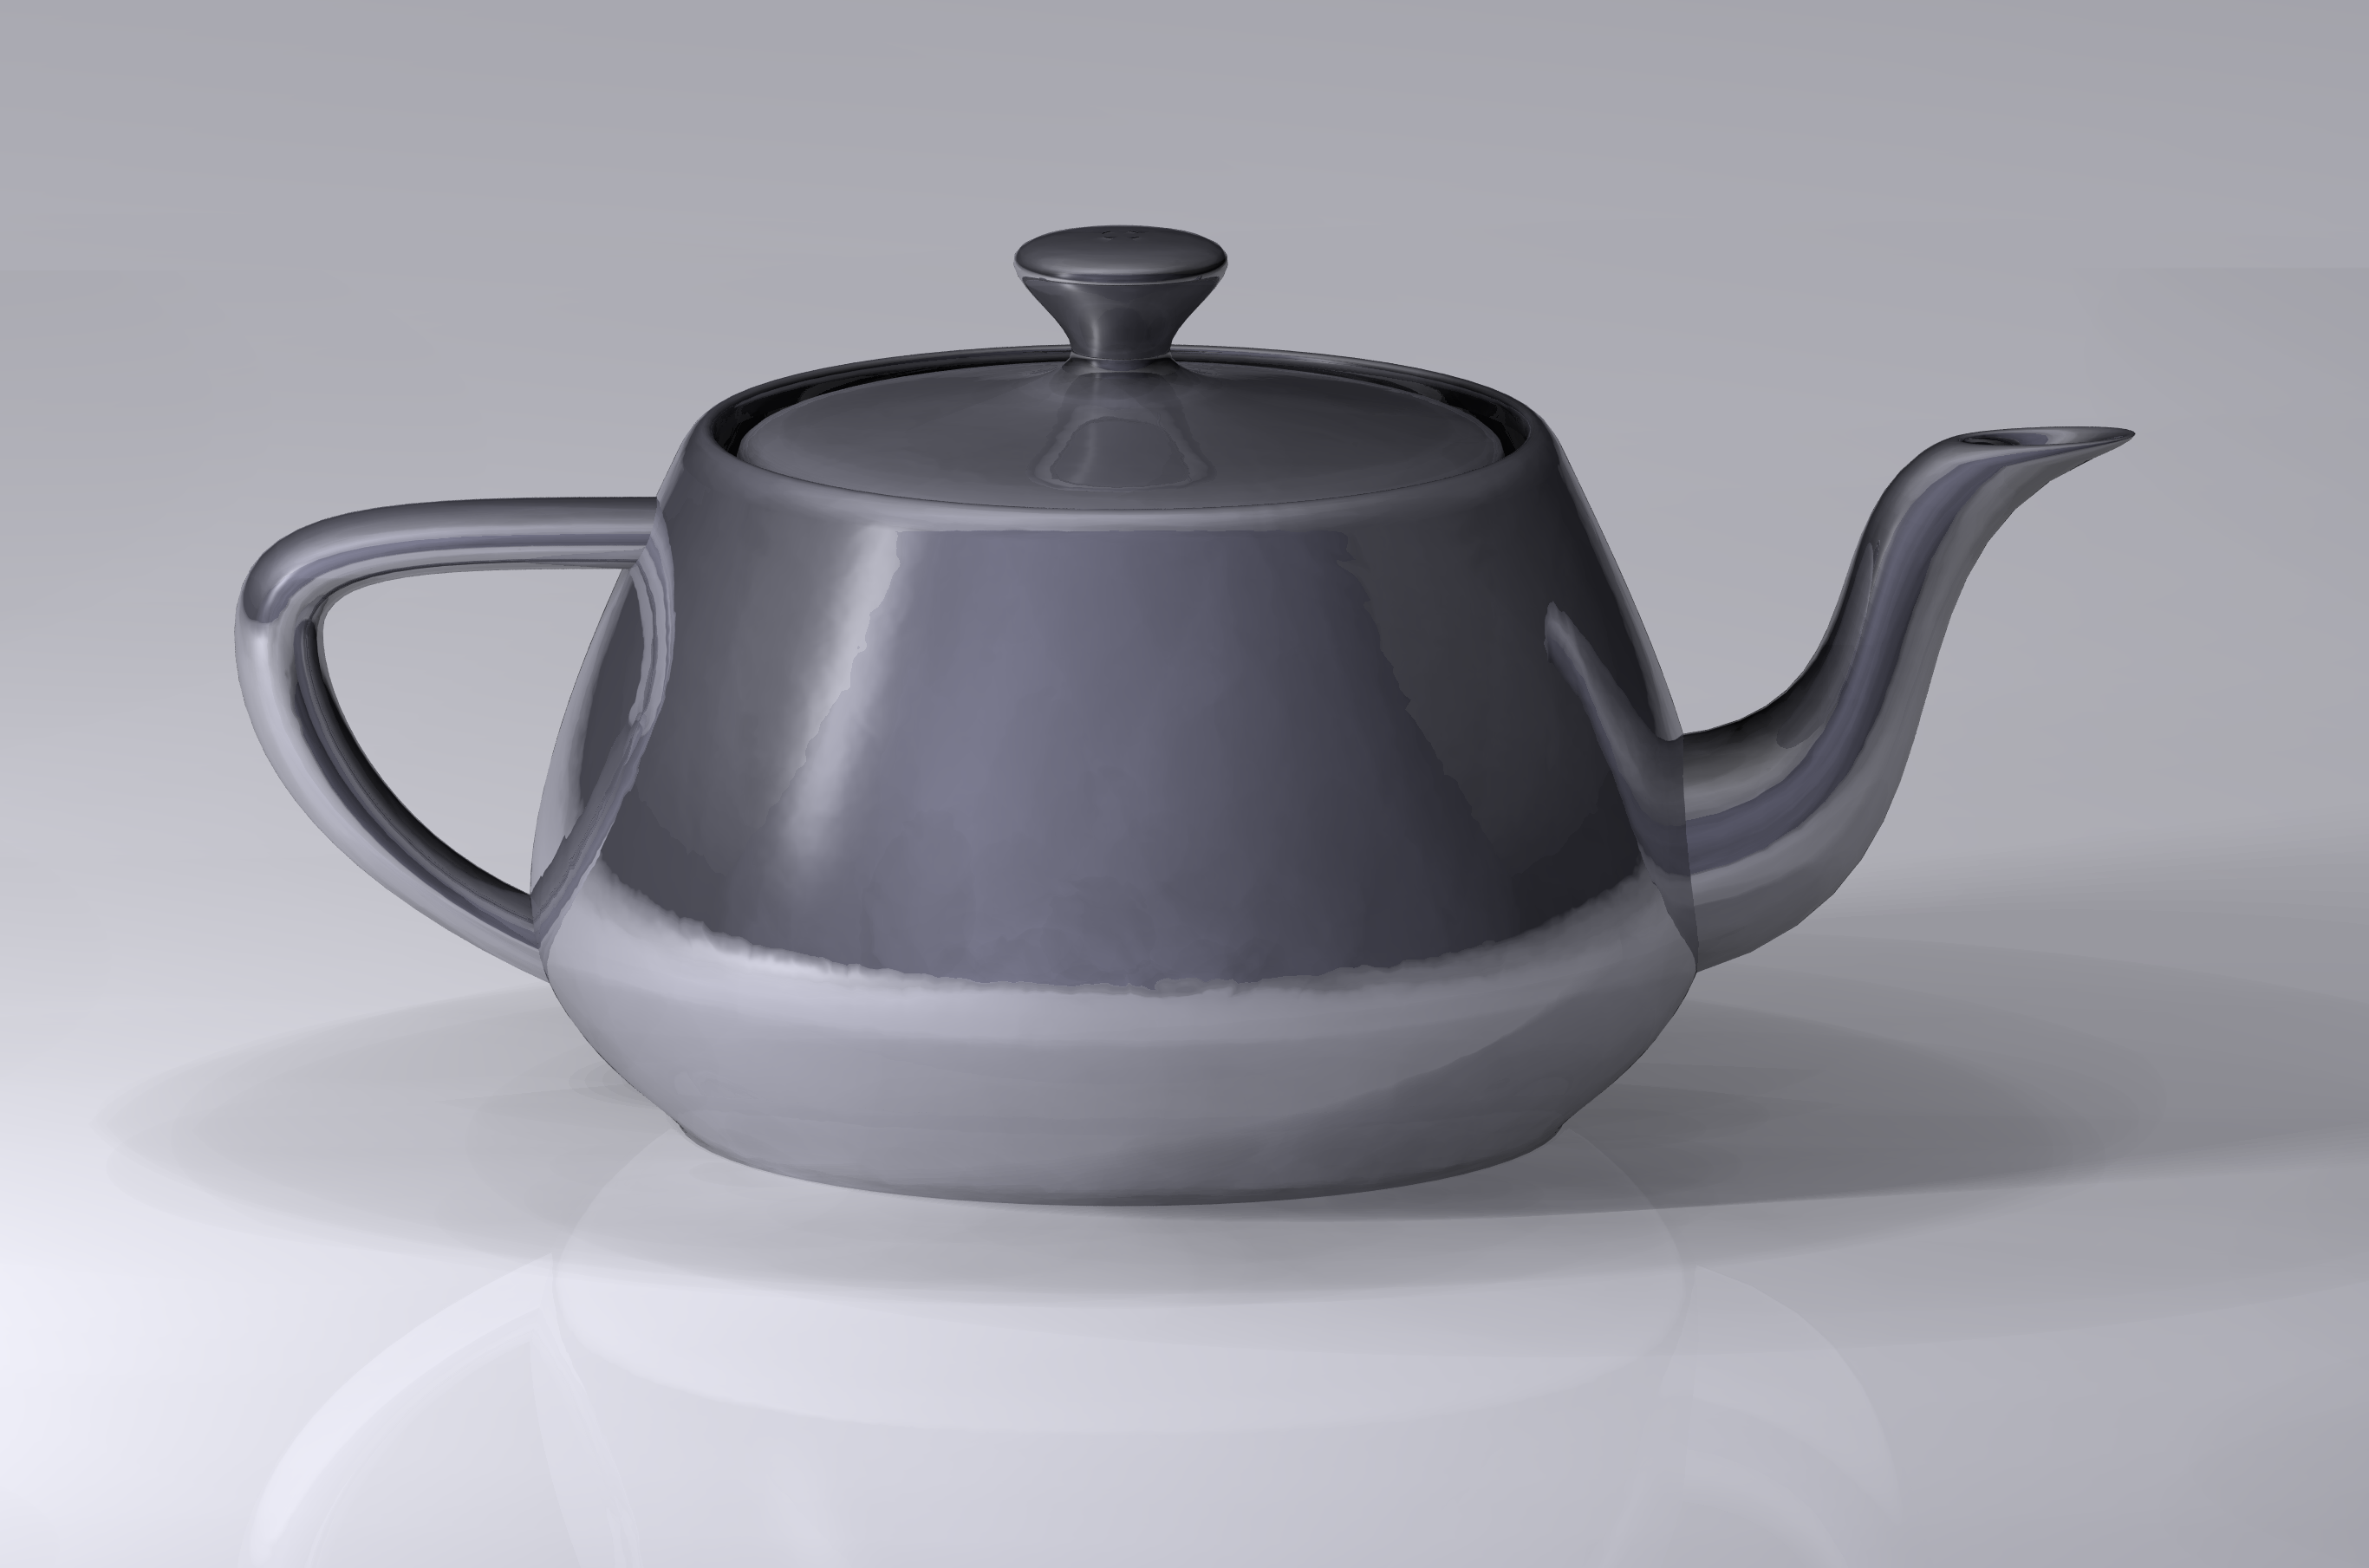
\includegraphics[scale=0.1]{images/Utah_teapot.png}
    \caption[Ein Rendering der Utah Teekanne]
            {Ein Rendering der Utah Teekanne, eines der weit verbreitetsten 
             3D-Modelle in der Computergrafik. 
             Sie wurde mit Bezierflächen modelliert.}
    \label{fig:rendering-utah-teapot}
\end{figure}



\section{Echtzeitvisualisierung und OpenGL}
\subsection{Geschichte}
OpenGL entstand ursprünglich aus dem von Silicon Graphics (SGI) entwickelten IRIS GL. Im sogenannten Fahrenheit-Projekt versuchten Microsoft und SGI ihre 3D-Standards zu vereinheitlichen, das Projekt wurde jedoch wegen finanzieller Schwierigkeiten auf Seiten von SGI abgebrochen.

Der OpenGL-Standard wird vom OpenGL ARB (Architecture Review Board) festgelegt. Das ARB existiert seit 1992 und besteht aus einer Reihe von Firmen. Stimmberechtigte Mitglieder sind die Firmen 3DLabs, Apple, AMD/ATI, Dell, IBM, Intel, Nvidia, SGI und Sun (Stand Nov. 2004). Weiter mitwirkende Firmen sind Evans and Sutherland, Imagination Technologies, Matrox, Quantum3D, S3 Graphics, Spinor GmbH, Tungsten Graphics, und Xi Graphics. Microsoft, eines der Gründungsmitglieder, hat das ARB im März 2003 verlassen.

Neue Funktionen in OpenGL werden meist zuerst als herstellerspezifische Erweiterungen eingeführt und gehen dann den Weg über herstellerübergreifende Erweiterungen und ARB-Erweiterungen zu Kernfunktionalität. Dies erlaubt es, neueste Möglichkeiten der Grafikhardware zu nutzen und dennoch OpenGL abstrakt genug zu halten.

Quelle: https://de.wikipedia.org/wiki/OpenGL
\subsection{GL-Pipeline}
Eine Computergrafik-Pipeline besteht im Wesentlichen aus den folgenden Schritten:
\begin{figure}[H]
    \centering
    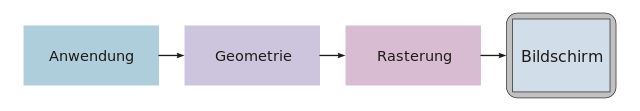
\includegraphics[width=1.0\textwidth]{images/cgpipeline_grob.png}
    \caption{Computergrafik-Pipeline}
    \label{fig:cdpipeline-overview}
\end{figure}

Eine solche Pipeline wird auch von OpenGL implementiert. Es besteht jedoch die Besonderheit, dass die Geometrie und die  Rasterung in Hardware realisiert ist und man durch kleine Programme, sogenannte Shader, auf diese Hardware zugreifen und Manipulationen vornehmen kann beziehungsweise seit OpenGL 2.0 sogar muss.



\subsubsection{Geometrie}
Die Geometrieverarbeitung   besteht aus der Hintereinanderausführung der folgenden affinen/homogenen Abbildungen und Algorithmen:
\begin{figure}[H]
    \centering
    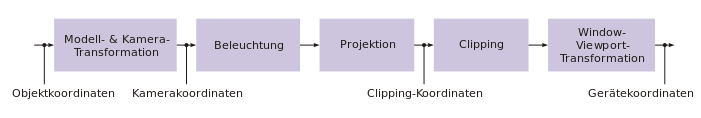
\includegraphics[width=1.0\textwidth]{images/cgpipeline.png}
    \caption{Geometrie-Pipeline}
    \label{fig:cgpipeline-geometry}
\end{figure}

\subsubsection*{Modell und Kameratransformationen}
Die Transformationen von Objektkoordinaten in das Kamerakoordinatensystem werden durch affine Transformationen beschrieben, welche durch Multiplikation durch homogene $4 \times 4$-Matrizen realisiert werden. 

\subsubsection*{Projektion}
Die Projektion wird durch Matrizen ähnlich der Projektionsmatrix 
$K_{persp_{xy}}$ und $K_{orth_{xy}}$ aus Abschnitt 
\ref{subsub:math:affine-space:homog-coords-projection} realisiert. 
Es werden jedoch noch  Translationen, Rotationen und Stauchungen 
dazwischen geschaltet, die ebenfalls als $4 \times 4$-Matrizen realisiert werden 
können und mit denen diese Matrix multipliziert werden. 
Man erreicht damit, dass der Kegelstumpf zwischen der vorderen 
(\textit{nearplane}) und der hinteren (\textit{farplane}) Projektionsebene in 
den $[-1,1] \times [-1,1] \times [-1,1] $ Würfel abgebildet wird, welcher auch 
Sichtvolumen genannt wird. 
\begin{figure}[H]
    \centering
    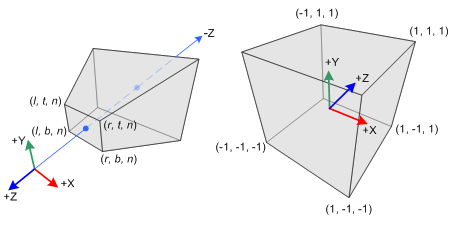
\includegraphics[width=1.0\textwidth]{images/gl_projectionmatrix01.png}
    \caption{Projektion und Sichtvolumen}
    \label{fig:projection-sight-vol}
\end{figure}

Die Multiplikation all diese Matrizen wird auch die MODEL-VIEW-PROJECTION-MATRIX genannt. 

In Fall obiger Grafik ist 
\begin{align*}
MVP := \begin{pmatrix}  
\frac{2n}{r-l}  &  0 &  \frac{r+l}{r-l}  & 0  \\
0   &  \frac{2n}{t-b} & \frac{t+b}{t-b} & 0  \\
0   &  0 & \frac{-f-n}{f-n} & \frac{-2\cdot f \cdot n}{f-n}  \\
0   &  0 & -1 & 0  
\end{pmatrix}  \; .
\end{align*} 
und insbesondere falls $r = -l$ und $t=-b$  ist

\begin{align*}
MVP := \begin{pmatrix}  
\frac{n}{r}  &  0 & 0  & 0  \\
0   &  \frac{n}{t} & \frac{t+b}{t-b} & 0  \\
0   &  0 & \frac{-f-n}{f-n} & \frac{-2\cdot f \cdot n}{f-n}  \\
0   &  0 & -1 & 0  
\end{pmatrix}  \; .
\end{align*} 

\subsubsection*{Windows-Viewport-Transformation}
Zuletzt müssen die zweidimensionalen Punkte noch mit Hilfe einer 
zweidimensionalen affinen Transformation in das Koordinatensystems des 
Anzeigenfensters auf dem Ausgabegerät transformiert werden. 
Diese Transformation wird auch Windows-Viewport-Transformation genannt.

\subsubsection{Rasterung}
\begin{figure}[H]
    \centering
    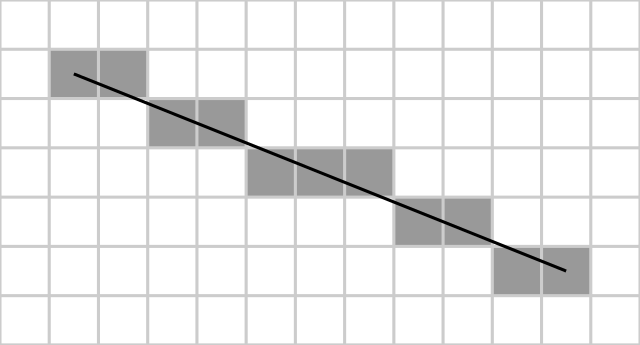
\includegraphics[width=1.0\textwidth]{images/bresenham.png}
    \caption{Rasterung nach Bresenham Algorithmus}
    \label{fig:screening-bresenham-line}
\end{figure}
Als Rasterung bezeichnet man das Transformieren kontinuierlicher, 
zweidimensionaler Daten auf diskrete Pixel. 
Anhand der gegebenen Daten muss also entschieden werden, welche Farbe ein Pixel des Ausgabegerätes erhält.
Wir haben also eine Funktion 
$Frame-Buffer: \mathbb{N} \times \mathbb{N} \to Farbe$. 
Im Bereich Echtzeitvisualisierung sind alle gängigen Rasterverfahren für 
Dreiecke und andere primitiven im wesentlichen Abwandlungen und 
Weiterentwicklungen von Algorithmen, die von Bresenham eingeführt wurden. 
Wir wollen uns den Bresenham Algorithmus für Linien/Strecken dazu exemplarisch 
anschauen.

\begin{Algorithmus}[Bresenham für Strecken mit positiver Steigung]
    \begin{figure}\centering
        \subfloat[Steigungsdreieck]{
            \begin{tikzpicture}[scale=1,]
                % axes
                \draw[->] (-.5, 0) -- (3, 0) coordinate (x axis);
                \node (x-label) at (x axis.south) [anchor=north] {$x$};
                \draw[->] (0, -.5) -- (0, 2) coordinate (y axis);
                \node (y-label) at (y axis.west) [anchor=east] {$y$};
                % S
                \draw[thick, black] (0.5, 0.5) coordinate (P) -- (2.5, 1.5) coordinate (Q);
                \filldraw [black] (P) circle (0.05cm);
                \node (P-label) at (P.west) [anchor=east] {$P$};
                \filldraw [black] (Q) circle (0.05cm);
                \node (Q-label) at (Q.east) [anchor=west] {$Q$};
                % triangle
                \draw[ultra thick, blue] (1, 3/4) -- ++(1, 0) coordinate (dx);
                \node (dx-label) at (dx.south west) [
                    anchor=north east, 
                    color=blue, 
                ] {$dx$};
                \draw[ultra thick, red] (dx) -- ++(0, 1/2) coordinate (dy);
                \node (dy-label) at (dy.south east) [
                    anchor=north west, 
                    color=red, 
                ] {$dy$};
                \draw[ultra thick, orange] (1, 3/4) -- ++(1, 1/2) coordinate (m);
                \node (m-label) at (m.west) [
                    anchor=south east, 
                    color=orange, 
                ] {$m = \frac{dy}{dx}$};
            \end{tikzpicture}
            \label{fig:screening-bresenham-triangle}
        }
        \hspace*{0.1\textwidth}
        \subfloat[Pixelraster]{
	\begin{tikzpicture}
                \foreach \x / \y / \pxname in {-1/-1/P, 0/-1/E, 0/0/N_E} {
                    \draw [lightgray, very thin] (\x, \y) rectangle ++(1, 1);
                    \ifthenelse{\x < 0}{
                        \node (\pxname) at (\x-.5, \y+.5) {$\pxname$};
                    }{
                        \node (\pxname) at (\x+1.5, \y+.5) {$\pxname$};
                    }
                }
                \filldraw [black] (0.5, 0) circle (0.05cm);
                \node (M_p) at (0.6, 0.2) {$M_p$};
                \filldraw [black] (-0.5, -0.5) circle (0.05cm);
		\draw[<-] [black, thin] (-0.55, -0.55) --(-1.6, -1.1);
                \node (x0_y0) at (-1.4, -1) [
                    anchor=north east, 
                    outer sep=0pt, 
                    xshift=0.4cm, 
                ] {$\left( x_p,~ y_p \right)$};
                \filldraw [black] (0.5, -0.5) circle (0.05cm);
		\draw[<-] [black, thin] (0.5, -0.6) --(0.5, -1.1);
                \node (x1_y0) at (0, -1) [
                    anchor=north west, 
                    outer sep=0pt, 
                    xshift=-0.4cm, 
                ] {$\left( x_p + 1,~ y_p \right)$};
       	\end{tikzpicture}
        \label{fig:screening-bresenham-pixels}
        }
        \caption{Schrittbetrachtung Bresenham Algorithmus}
        \label{fig:screening-bresenham}
    \end{figure}
    Die Strecke $S = \overline{PQ} \in \mathbb{R}^n$ soll auf ein 
    ($n$-dimensionales Pixel-) Raster abgebildet werden (Siehe Abbildung 
    \ref{fig:screening-bresenham-line}). 
    Wir beschränken uns hier auf die Berechnung im $\mathbb{R}^2$. 
    $P$ und $Q$ seien gegeben mit 
    \begin{equation*}\begin{matrix}
        P = \begin{pmatrix} x_0 \\ y_0 \end{pmatrix} & 
        Q = \begin{pmatrix} x_1 \\ y_1 \end{pmatrix} & 
        \forall x_i, y_i \in \mathbb{R}
    \end{matrix}\end{equation*}
    Die Geradengleichung lässt sich einfach bestimmen (Abbildung 
    \ref{fig:screening-bresenham-triangle}):
    \begin{equation*}\begin{matrix}
        y & = & mx + b \\
        & \textrm{mit} & \\
        m & = & \frac{dy}{dx} \\
        dx & = & x_1 - x_0 \\
        dy & = & y_1 - y_0 \\
    \end{matrix}\end{equation*}
    Die Abbildung auf ein Raster ist für Steigungen 
    $m \in \left\{ 0,~ 1 \right\}$ trivial. 
    Anders für $0 < m < 1$. 
    Dafür betrachten wir in einem Schritt benachbarte Pixel 
    (Abbildung \vref{fig:screening-bresenham-pixels}): 
    \begin{itemize}
        \item Ausgangspixel $P\left( x_p,~ y_p \right)$
        \item Nachbar $E\left( x_p + 1,~ y_p \right)$
        \item ,,Nachfolgender'' Nachbar $N_E\left( x_p + 1,~ y_p + 1 \right)$
    \end{itemize}
    Der Mittelpunkt zwischen $N$ und $E$ wird festgelegt durch
    \begin{equation*}
        M_p = \left( x_p + 1,~ y_p + \frac{1}{2} \right)
    \end{equation*}
    Damit kann entschieden werden welches benachbarte Pixel zur Strecke gehört. 
    Liegt nun
    \begin{equation*}
        M_p ~\Big\{~ \begin{matrix}
            \textrm{oberhalb}~ \overline{PQ} &\Rightarrow& \textrm{wähle}~ E \\ 
            \textrm{unterhalb}~ \overline{PQ} &\Rightarrow& \textrm{wähle}~ N_E 
        \end{matrix}
    \end{equation*}\\
    Bresenham hat eine effiziente Lösung dieses Problems aufgezeigt.
    Zunächst lässt sich die Geradengleichung in eine Funktion $F$ umformen, die von 
    zwei Variablen abhängt: 
    \begin{equation*}\begin{matrix}
        y & = & \frac{dy}{dx} x + b \\
        dx \cdot y & = & dy \cdot x + dx \cdot b \\
        0 & = & dy \cdot x - dx \cdot y + dx \cdot b \\
        F\left(x,~ y\right) & := & dy \cdot x - dx \cdot y + dx \cdot b 
    \end{matrix}\end{equation*}
    Das arithmetische Entscheidungskriterium lautet also 
    \begin{equation*}\begin{matrix}
        (x,~ y) \in y = mx + b & \Leftrightarrow & F\left(x,~ y\right) = 0 \\
        & \textrm{bzw.} & \\
        F\left(x,~ y\right) & \Bigg\{ & \begin{matrix}
            = 0 & \left(x,~ y\right) \textrm{liegt auf}~ S \\
            > 0 & \left(x,~ y\right) \textrm{liegt unterhalb von}~ S \\
            < 0 & \left(x,~ y\right) \textrm{liegt oberhalb von}~ S \\
        \end{matrix}
    \end{matrix}\end{equation*}
    Damit kann die Entscheidungsfunktion $D_p$ definiert werden 
    \begin{equation*}\begin{matrix}
        D_p & := & 2 \cdot F\left(M_p\right) \\
        & = & 2 \cdot F\left(x_p + 1,~ y_p + \frac{1}{2}\right) \\
        & = & dy \left(2x_p + 2\right) - dx \left(2y_p + 1\right) + dx \cdot 2b
    \end{matrix}\end{equation*}
    1. Fall: $D_p < 0 ~\Rightarrow~$ Nachfolgepixel ist $E$
    \begin{equation*}\begin{matrix}
        D_E & = & 2 \cdot F\left(M_E\right) \\
        & = & 2 \cdot F\left(x_p + 2,~ y_p + \frac{1}{2}\right) \\
        & = & dy \cdot \left(2 x_p + 4\right) 
            - dx \cdot \left(2 y_p + 1\right) 
            + 2 \cdot b \cdot dx \\
        & = & D_p + \bigtriangleup_E \\
        & \textrm{mit} & \bigtriangleup_E := 2 \cdot dy
    \end{matrix}\end{equation*}
    2. Fall: $D_p \ge 0 ~\Rightarrow~$ Nachfolgepixel ist $NE$ \\
    \begin{equation*}\begin{matrix}
        D_{NE} & = & 2 \cdot F\left( M_{NE} \right) \\
        & = & D_p + \bigtriangleup_{NE} \\
        & \textrm{mit} & \bigtriangleup_{NE} := 2dy - 2dx
    \end{matrix}\end{equation*}
    Eine Implementierung könnte wie folgt aussehen: 
    \begin{lstlisting}[language=C]
bresenham(x0, y0, x1, y1){
    dx = x1 - x0;
    dy = y1 - y0;
    d = 2*dy - dx; /*F(x0 + 1,y0 + 1/2) | F(x0,y0)=0*/
    deltaE = 2 * dy;
    deltaNE = 2 * (dy - dx);
    x = x0;
    y = y0;
    writepixel(x0, y0);
    while (x < x1) {
        if (d < 0) {
            d += deltaE;
            x++;
        } else {
            d += deltaNE;
            x++; y++;
        }
        writepixel(x, y);
    }
}
    \end{lstlisting}
\end{Algorithmus}

Das Rastern erzeugt oft harte, kantige und ausgefranste Übergange. Diese Effekte bezeichnet man auch als Aliasing. Algorithmen, die diesen Aliasing-Effekten entgegenwirken nennt man auch 
Antialiasing. 
\begin{figure}[H]
    \centering
    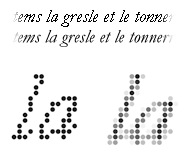
\includegraphics[width=0.5\textwidth]{images/Antialiasing.png}
    \caption{Eine Schrift mit und ohne Antialiasing}
    \label{fig:screening-antialiasing-font}
\end{figure}


\subsection*{Sichtbarkeitsprobleme}

\subsubsection*{Clipping}
Beim 3D-Clipping werden alle Polygone verworfen, die nach der Transformation in Clipping-Koordinaten vollständig ausserhalb des Sichtvolumens
$[-1,1] \times [-1,1] \times [-1,1] $ liegen. Das 2D-Clipping findet nach der Projektion der Polygone statt. Polygone, die über das Viewportfenster hinaus ragen, werden an den Fensterkanten abgeschnitten.
Der wichtigste Schritt ist hierbei das Abschneiden von Strecken an diesen Kanten. Wir betrachten dazu exemplarisch den Cohen-Sutherland-Algorithmus:

\begin{Algorithmus}[Cohen-Sutherland]
\end{Algorithmus}

\subsubsection*{Culling/Rückseitenentfernung}
Als Culling bezeichnet man das Entfernen von Polygonen anhand Ihrer Orientierung, beziehungsweise Anhand der zugehörigen Normale. Man definiert, welche Orientierung eine Rückseite darstellt und verwirft dann Polygone, deren Normale positives beziehungsweise negatives Skalarprodukt mit der Blickrichtung aufweisen. So werden Beispielsweise Rückseiten, die nicht sichtbar sind, nicht weiter in der Pipeline verarbeitet.

\subsubsection* {z-Buffer}
Der Z-Buffer enthält für jedes Pixel $(u,v)$ nach der Rasterung  einen Wert zwischen $-1$ und $1$. Dieser Wert  ist der Abstand zum nächsten Punkt eines Polygons  in Clipping-Koordinaten von diesem Pixel auf der Projektionsebene.  Wir haben somit eine Funktion
\begin{align*}
Z-Buffer : \mathbb{N} \times \mathbb{N} \to [-1,1]  \; .
\end{align*}

\begin{figure}[H]
    \centering
    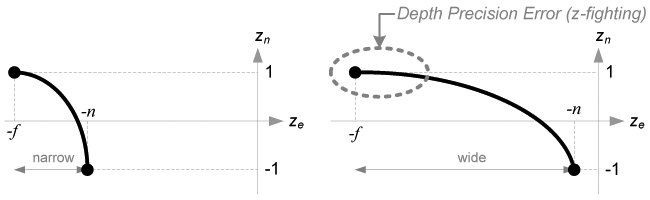
\includegraphics[width=1.0\textwidth]{images/gl_projectionmatrix_zbuffer_1.png}
    \caption{Z-Buffer-War}
    \label{fig:zbuffer-war}
\end{figure}



\begin{Algorithmus}[z-Buffer Algorithmus]
Setze Alle Einträge im Z-Buffer auf 1 (Hintergrund).
Setze alle Einträge im Framebuffer auf die Hintergrundfarbe. \\
$\forall$ Polygone P: \\
begin: \\
Transformiere das Polygon in Clipping-Koordinaten. \\
Transformiere das Polygon in Rasterkoordinaten. \\
$\forall$ erhaltenen Pixel (u,v): \\
begin: \\
$pz := $Z-Koordinate des Polygons in Clipping-Koordinaten zum entsprechenden Pixel \\
$zz:=$ Eintrag im Z-Buffer für das Pixel $(u,v)$ \\
if $pz < zz$: \\
begin: \\
$Z-Buffer(u,v) := pz$ \\
$Frame-Buffer(u,v) := Farbe(P,(u,v))$ \\
end \\
end \\
end
\end{Algorithmus}


\subsection{Lokale Beleuchtungsmodelle}
\subsubsection{Ideale und diffuse Reflexionen}
\subsubsection{Lambert  Modell}
Das Lambertsche Modell beschreibt, wie durch den perspektivischen Effekt die Strahlungsstärke mit flacher werdendem Abstrahlwinkel abnimmt. Sei nun $L$ der Punkt, an dem sich eine punktförmige Lichtquelle befindet und $P \in N$ ein Punkt eines Netzes $N$ mit Normale $n$ (also insbesondere gilt $||n|| = 1$).  Dann berechnet sich die Lichtintensität $I_d$ an diesem Punkt durch
\begin{align*}
I_d :=  I_l \cdot I_m \cdot max\biggl ( 0, \biggl< n, \frac{1}{||\overline{PL}||} \cdot \overline{PL} \biggr> \biggr)
\end{align*}
wobei $I_l \in [0,1]$ die Lichtintensität der Lichtquelle, $I_m \in [0,1]$ eine Materialkonstante und $max(a,b)$ das maximum der Zahlen $a$ und $b$ ist. 
Um die gesamte Lichtintensität zu berechnen wird noch ein konstanter, sogenannter ambienter Lichtanteil $I_a$ hinzuaddiert
\begin{align}
I := I_d + I_a \;.
\end{align} 
$I_a$ ist wie gesagt eine Konstante.
 Der Eindruck von ambienten Licht, also Licht, das aus keiner erkennbaren Richtung kommt und alles gleichmässig erhellt, entsteht durch Lichtstrahlen, die sehr oft an Gegenständen reflektiert werden.
Der Wert $I$ muss gegebenenfalls auf das Intervall $[0,1]$ beschränkt werden.
\begin{figure}[H]
    \centering
    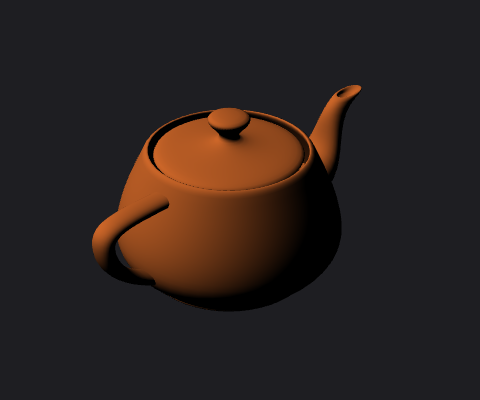
\includegraphics[width=0.8\textwidth]{images/lambert.png}
    \caption{Lambert Modell diffuser Reflektion}
    \label{fig:reflection-lambert-diffuse-model}
\end{figure}

   
\subsubsection{Phong Modell}
Das Phong-Modell erweitert das  Lambert-Modell um den Effekt von spiegelnden Reflektionen. Die Idee ist, dass die Helligkeit zusätzlich zunimmt, je mehr die Betrachtungsrichtung dem perfekt reflektiertem Lichtstrahl entspricht.  

\begin{figure}[H]
    \centering
    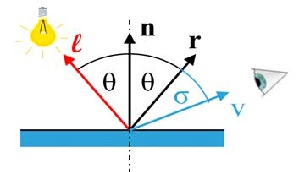
\includegraphics[width=0.6\textwidth]{images/phong_directions.jpg}
    \caption{Die einzelnen Komponenten des Phong-Modells}
    \label{fig:phong-directions}
\end{figure}

Ist $v$ der normierte Vektor in Richtung Kamera und $l$ der normierte Vektor in Richtung Lichtquelle, dann definiert man die  reflektierende Lichtintensität durch
\begin{align}
I_s := I_l \cdot I_m \cdot s \cdot \max\biggl ( 0, <r,v>^h \biggr)\;.
\end{align}
$I_l$ ist hierbei wieder die Intensität der Lichtquelle und $I_m$ eine Materialkonstante. Beide liegen in einen Wertebereich von $[0,1]$ 
$h$ ist eine ganze Zahl im Wertebereich $[0, \infty)$ und bestimmt die "härte" der Reflexion. $s$ ist eine Fließkommazahl im Wertebereich $(0,1]$ und beeinflusst den Glanz der Oberfläche.
 Der Vektor $r$ lässt sich berechnen durch 
\begin{align}
r = -l + 2 \cdot <n, l> \cdot n
\end{align}
wobei $n$ die Normale an dem betrachteten Oberflächenpunkt ist.

\begin{figure}[H]
    \centering
    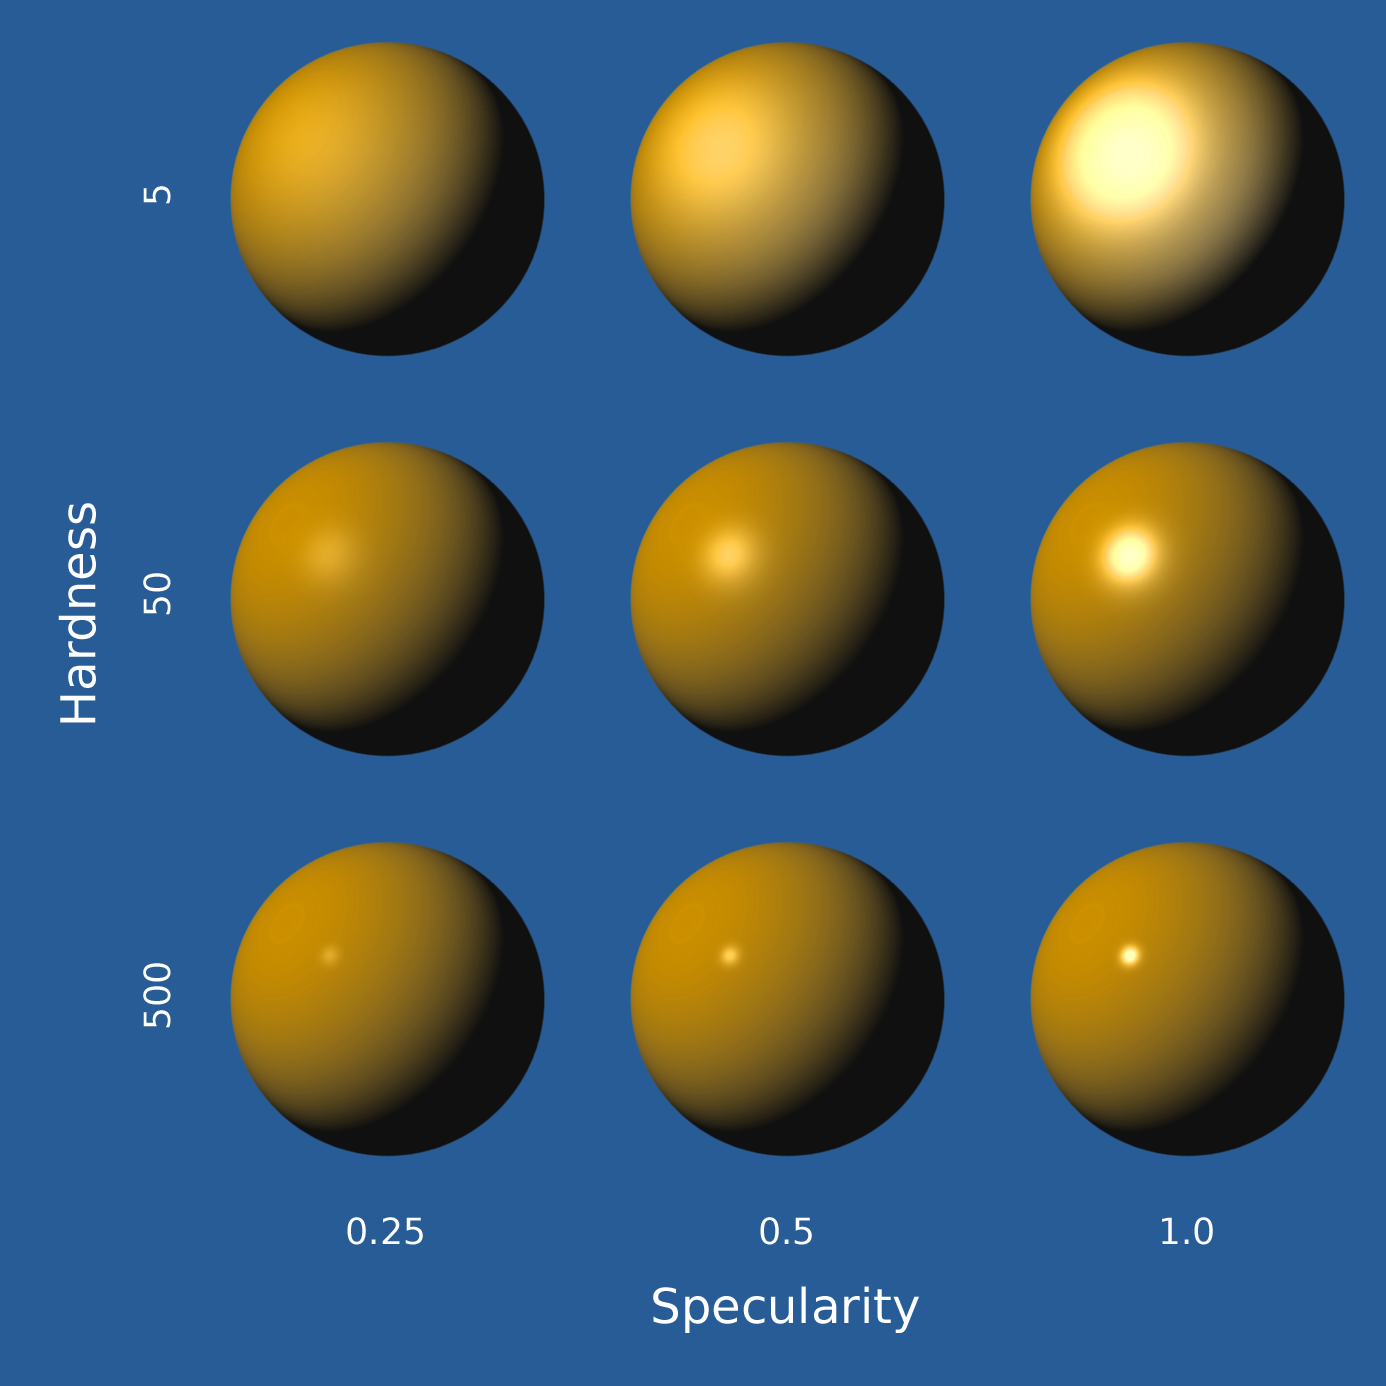
\includegraphics[width=0.8\textwidth]{images/phong.png}
    \caption{Phong Modell spiegelnder Reflektion}
    \label{fig:reflection-phong-specular-model}
\end{figure}

Im Phong-Modell wird nun die endgültige Lichtentität wie folgt zusammengesetzt:

\begin{align}
I := I_s + I_d + I_a
\end{align}
wobei $I_d$ die diffuse Lichtintensität aus dem Lambert-Modell und $I_a$ den konstanten, ambienten Anteil bedeutet.
Gegebenenfalls muss $I$ wieder auf das Intervall $[0,1]$ beschränkt werden.

\begin{figure}[H]
    \centering
    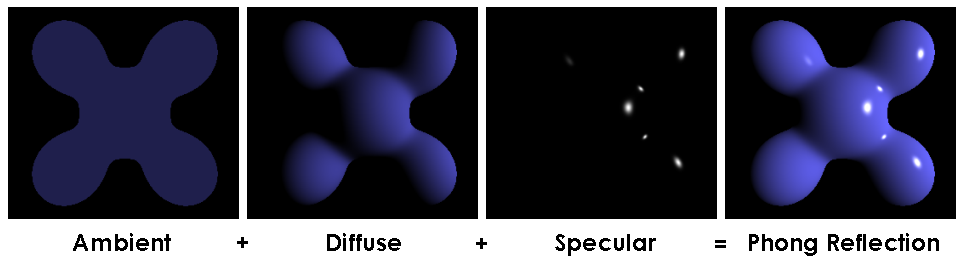
\includegraphics[width=1.0\textwidth]{images/Phong_Components.png}
    \caption{Die einzelnen Komponenten des Phong-Modells}
    \label{fig:phong-components}\end{figure}

Die Möglichkeiten, ein bestimmtes Material zu beschreiben, sind  beim Phong-Modell beschränkt. 
Es gibt komplexere lokale Beleuchtungsmodelle, wie zum Beispiel das Cook-Torrente-Modell, die eine detaillierte Materialbeschreibung zulassen.




\subsection{Shader und standard Algorithmen}

\subsubsection{Flat-Shading}
\begin{figure}[H]
    \centering
    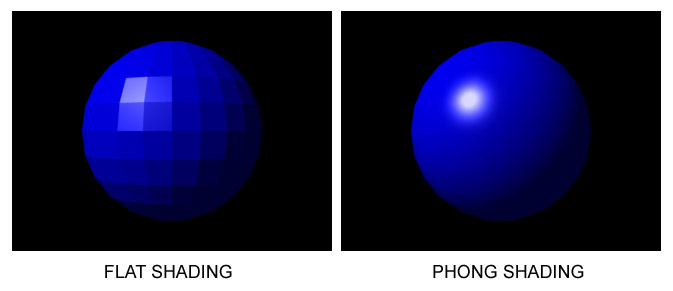
\includegraphics[width=1.0\textwidth]{images/phong_flat_shading.jpg}
    \caption{Flat- und Phong-Shading-Modelle}
    \label{fig:shading-flat-phong-models}
\end{figure}


\subsubsection{Gouraud und Phong Shading}
\begin{figure}[H]
    \centering
    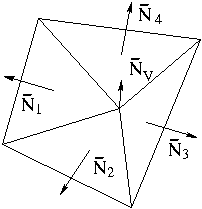
\includegraphics[width=0.5\textwidth]{images/gouraud_normals.png}
    \caption{Verschiedene Normalen von angrenzenden Flächen}
    \label{fig:gouraud-shading-scanline}
\end{figure}

\begin{figure}[H]
    \centering
    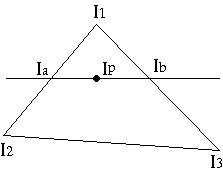
\includegraphics[width=0.5\textwidth]{images/gouraud_scanline.png}
    \caption{Scanline-Verfahren beim Gouraud-Shading}
    \label{fig:gouraud-shading-scanline}
\end{figure}



\subsubsection{Texturen und UV-Mapping}
\begin{figure}[H]
    \centering
    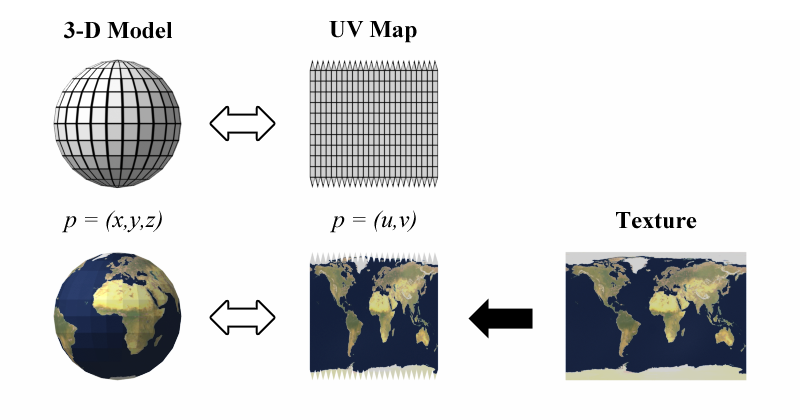
\includegraphics[width=1.0\textwidth]{images/tm_uv.png}
    \caption{uv mapping} %TODO: fix caption&label
    \label{fig:uv-mapping1}
\end{figure}

\begin{figure}[H]
    \centering
    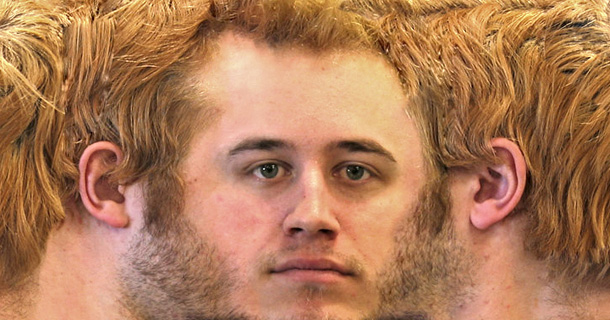
\includegraphics[width=1.0\textwidth]{images/tm_face.jpg}
    \caption{uv mapping} %TODO: fix caption&label
    \label{fig:uv-mapping2}
\end{figure}




\subsubsection{Bumpmapping}
Die relativen Höheninformationen liegen in einer Textur in Form von Graustufen vor – der sogenannten Heightmap. Jeder Grauwert steht für eine bestimmte Höhe. Normalerweise ist Schwarz (Wert 0) die „tiefste“ Stelle und Weiß (Wert: 255) die „höchste“.  Bei der Lichtberechnung, die wesentlich von der Normale abhängt, wird die gegebene Normale so abgeändert, als gäbe es eine Vertiefung bzw. eine Erhöhung entsprechend der Höheninformation.  Da Höhenunterschiede nur durch Veränderung der Helligkeit vorgegaukelt werden, die Flächen aber glatt bleiben, treten einige sichtbare Fehler auf:
Bei flachem Betrachtungswinkel wirkt die Struktur stark verzerrt.
Die Silhouette bleibt so eben wie beim ursprünglichen Objekt.
Es wird ein glatter Schatten geworfen.
Bumps werfen keine Schatten aufeinander.
\subsubsection{Bumpmapping}
\begin{figure}[H]
    \centering
    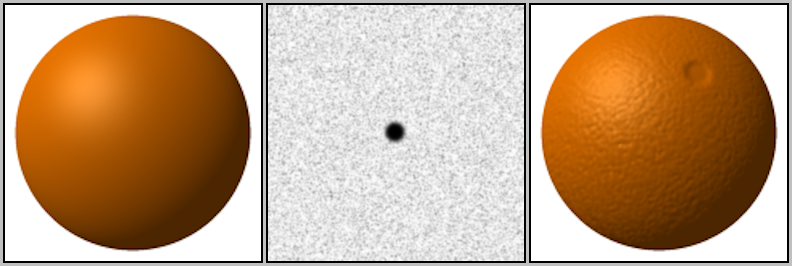
\includegraphics[width=1.0\textwidth]{images/Bumpmap.png}
    \caption{uv mapping} %TODO: fix caption&label
    \label{fig:uv-mapping3}
\end{figure}




\subsubsection{Displacementmapping}
Wie beim Bumpmapping  wird  eine Height-map als Textur mitgegeben.
Im Gegensatz dazu werden die Punkte des Gitternetzes (Vertices)  entsprechend diesen Texturinformationen entlang ihrer Normalen, das heißt senkrecht zur Oberfläche, tatsächlich verschoben. So ist es beispielsweise möglich, ein Höhenrelief durch das Anwenden einer Displacement Map auf eine ebene (planare) Oberfläche zu übertragen und dieser damit eine raue Struktur zu verleihen. Zusätzlich zur Verschiebung kann in Abhängigkeit von der Dichte des Drahtgitters dessen Verfeinerung notwendig werden. Man spricht dann von Tesselation.

\begin{figure}[H]
    \centering
    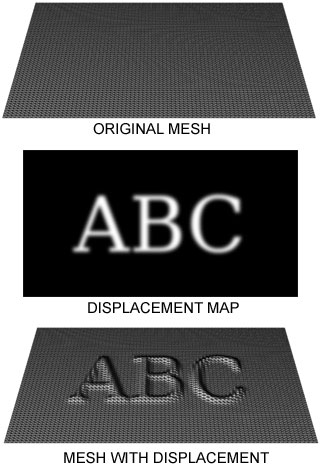
\includegraphics[width=0.5\textwidth]{images/Displacement.jpg}
    \caption{Displacementmapping} %TODO: fix caption&label
    \label{fig:displacement-mapping}
\end{figure}



\subsubsection{Shadowmap}
Das Rendern einer Szene mit Schatten unter Zuhilfenahme von einer Shadow Map geschieht im Wesentlichen in zwei Schritten. Als erstes wird die Szene aus der Sicht des Lichts gerendert und die Tiefeninformation (z-Buffer) in eine Textur gerendert. Anschließend wird die Szene normal gerendert, wobei für jedes Pixel  der Abstand des zugehörigen Vertex zur Lichtquelle (in Clipping Coordinaten) mit dem Wert der Shadow Map verglichen wird. Ist der Wert in der Shadow Map kleiner, wird  das Pixel schattiert gerendert.

\begin{figure}[H]\centering
    \subfloat[Tiefeninformation aus Sicht des Lichtes gerendert]{
        \hspace*{0.05\textwidth}
         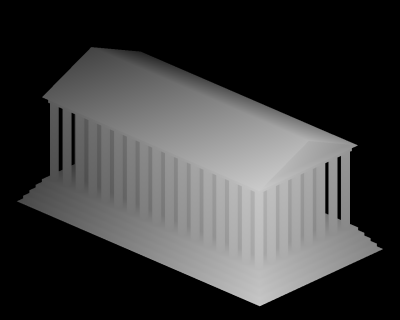
\includegraphics[width=0.5\textwidth]{images/sm_zb.png}
    \label{fig:shadowmap3}
    }
    \hspace*{0.1\textwidth}
    \subfloat[Rendering ohne Shadow mapt]{
        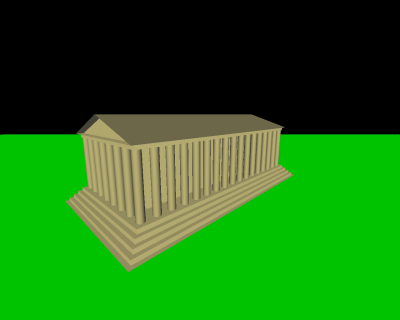
\includegraphics[width=0.5\textwidth]{images/sm_ns.png}
    \label{fig:shadowmap1}
    }
    \vspace*{1em}
    \subfloat[Rendering mit Shadow map]{
        \hspace*{0.05\textwidth}
         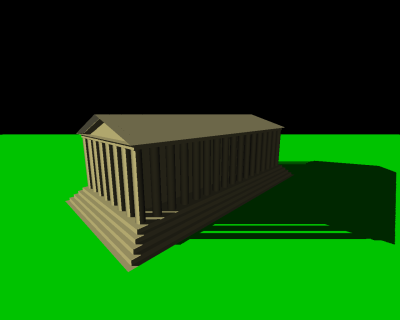
\includegraphics[width=0.5\textwidth]{images/sm_ws.png}
    \label{fig:shadowmap2}
    }
\end{figure}



Probleme bereitet der sogenannte z-Buffer War. Abhilfe schafft eine transformation der z-Buffer-Werte durch eine geeignete Funktion.



\subsubsection{ Forward shading, Blending und Transparenz}
Beim Forward shading wird die Lichtberechnung für jedes Vertex in dem entsprechen shader durchgeführt. Im Gegensatz dazu vergleiche deferred shading.
Werden mehrere Render passes durchgeführt, so kann man über das Blending festlegen, wie die doppelten Fragmente gemischt werden.
Transparenz kann man zum Beispiel realisieren, indem man die transparenten Objekte mit entsprechendem Blending über die vorher gerenderten  Szene rendert.
Ein lineares Blending wird zum Beispiel durch die Funktion 
\begin{align}
p_{neu} = \alpha \cdot p_1 + (1- \alpha)p_2
\end{align}
realisiert. Mehrere Lichtquellen können entweder direkt im Shader oder durch mehrfaches Rendern der Szene mit den verschiedenen Lichtquellen und entsprechendem Blending realisiert werden.
\subsubsection{Deferred shading}
Der Begriff Deferred Shading (zu dt. "verzögertes Schattieren") oder auch Deferred Lighting ("verzögerte Beleuchtung") beschreibt eine Technik, mit deren Hilfe die Geometrieverarbeitung von der Lichtberechnung getrennt werden kann. Dies erlaubt hunderte Lichtquellen in einer hoch-komplexen Szene.


Um eine Szene mit einem traditionellen Forward-Renderer zu beleuchten, wird normalerweise jedes Objekt der Szene mit den entsprechenden Beleuchtungsparametern der Lichtquelle gezeichnet. 
Die Lichtberechnungen werden für jedes Vertex aufgerufen.

Deferred Shading verfolgt einen anderen Ansatz: Für jeden Pixel werden die Daten aus dem G-Buffer ausgelesen und die Beleuchtung entsprechend dieser Daten im Fragmentshader einer minimalen, bildschirmfüllenden Geometrie berechnet. 


\begin{figure}[H]
    \centering
    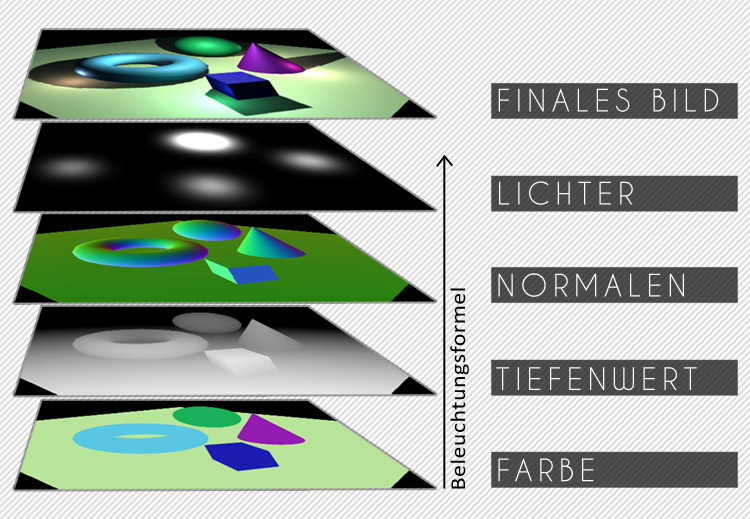
\includegraphics[width=1.0\textwidth]{images/deffered_shading.jpg}
    \caption{G-Buffer beim deferred shading} %TODO: fix caption&label
    \label{fig:defferedshading}
\end{figure} 

Mit dieser Methode sind hunderte Lichter gleichzeitig in einer hoch-komplexen Szene möglich.
Der Vorteil ist, dass die Lichtberechnungen somit nur für wirklich sichtbaren Pixel des tatsächlichen Ausgebe-Bildes  berechnet werden.
Das Verfahren ist nur dann sinnvoll, wenn man es mit einer sehr komplexen Geometrie und sehr vielen Lichtquellen zu tun hat. 

\begin{figure}[H]
    \centering
    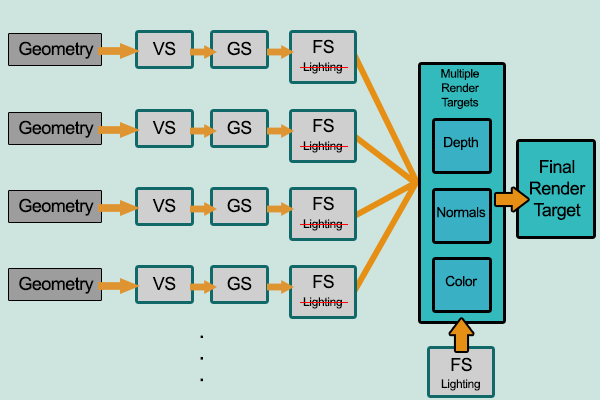
\includegraphics[width=0.8\textwidth]{images/deferred_v2.png}
    \caption{Pipeline beim deferred rendering} %TODO: fix caption&label
    \label{fig:defferedshading}
\end{figure}



\begin{figure}[H]
    \centering
    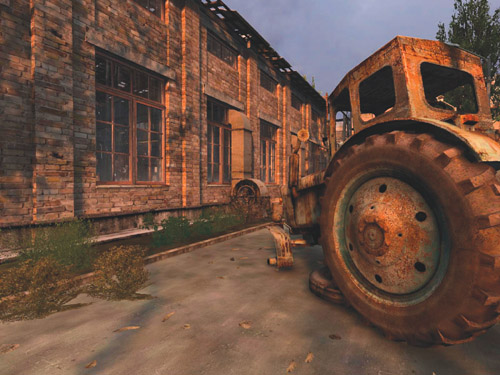
\includegraphics[width=0.8\textwidth]{images/deferred_shading_off.jpg}
    \caption{Szene gerendert mit forward shading. } %TODO: fix caption&label
    \label{fig:defferedshading}
\end{figure}



\begin{figure}[H]
    \centering
    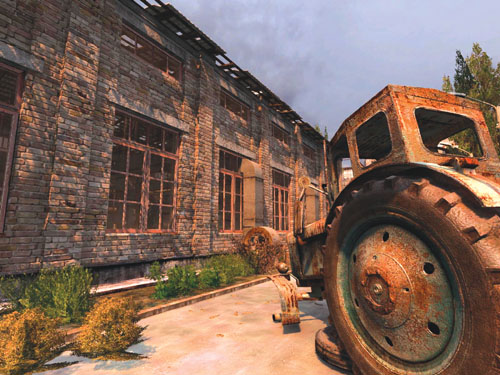
\includegraphics[width=0.8\textwidth]{images/deferred_shading_on.jpg}
    \caption{Szene gerendert mit  diferred shading. Der verbesserte  Eindruck des Tageslichtes wird durch eine sehr hohe Anzahl von Lichtquellen erzeugt.} %TODO: fix caption&label
    \label{fig:defferedshading}
\end{figure}



\subsection{GLSL via WebGL}

\section{Raytracing}

\subsection{Farbwahrnehmung und Farbmodelle}
\subsection{Globale Beleuchtungsmodelle und Rendergleichung}
\subsubsection{Radiometrie}
Die Radiantenergie $Q$ ist die Lichtenergie. Sie wird durch einen Strom von Photonen erzeugt. Die Energie eines Photons ist 
durch $E=h \cdot f$ geben, wobei $h$ das konstante Planksche Wirkungsquantum und $f$ die Frequenz der (Licht) Welle ist.  
Die Ableitung nach der Zeit
\begin{align}
\phi := \frac{\partial Q}{\partial t}
\end{align}
wird als Radiant Flux oder Strahlungsleistung bezeichnet. Diese  beschreibt den Energiefluss, beziehungsweise den Energie-Eintritt und Energie-Austritt.
Der Radiant Flux in einem infinitesimal dünnen Strahl vom Punkt $x$ in Richtung $\omega$ wird als Radiance $L(x, \omega)$ bezeichnet was  Formal durch
\begin{align}
L(x, \omega) := \frac{d^2Q}{\cos(\theta) dA \cdot d\omega}
\end{align}
ausgedrückt wird. Die Radiance ist also der Radiant Flux pro infinitesimale Flächeneinheit $\cos(\theta) dA$ und pro  Raumwinkel $d \omega$.
\subsubsection{BRDF und Reflectancegleichung }
Die sogenannte bidirektionale Reflektanzverteilungsfunktion (engl. Bidirectional Reflectance Distribution Function, BRDF)
ist eine Funktion $f_r (x, \omega_i, \omega_r)$, die das Reflexionsverhalten der Oberfläche eines Materials beschreibt. 
Sie hat als Eingabe die ausgehende Richtung $\omega_r$ und die eingehende Richtung  $\omega_i$ am Punkt $x$. 
Sie  liefert den Quotienten aus Strahlungsdichte und Bestrahlungsstärke für die ausgehende Richtung $\omega_r$ und die eingehende Richtung  $\omega_i$ am Punkt $x$.
Sie gibt somit die Abhängigkeit des reflektierten Lichts von der einfallenden Lichtstärke an: 
\begin{align}
dL_r = f_r(x, \omega_i, \omega_r) dE =   f_r(x, \omega_i, \omega_r) L_i(x,\omega_i) \cos(\theta_i) d \omega_i\\
L_r(x, \omega_r) = \int_{H^2} dL_r =    \int_{H^2}f_r (x, \omega_i, \omega_r) \cdot L(x, \omega_i) \cos(\theta_i) d\omega_i
\end{align}
Letztere Gleichung wird auch Reflectance-Gleichung genannt.
 \begin{figure}[H]
    \centering
    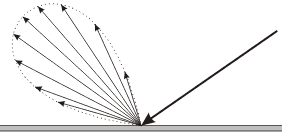
\includegraphics[width=0.6\textwidth]{images/brdf2.png}
    \caption{BRDF Funktion}
    \label{fig:raytracin_brdf}
\end{figure}

 
\subsubsection{Die Rendergleichung (Erste und zweite Form)}

\subsection{Raycasting}
\subsubsection{"Klassisches" Raytracing}
\subsubsection{Monte Carlo Integration und Pathtracing}
\subsubsection{Datenstrukturen für Bereichsabfragen}

\subsection{Raymarching}
\subsection{Labor}
\subsubsection{Blender}
\subsubsection{Echtzeitfähiges Raymarching in WebGL}

\section{Animation und Simulation}
\subsection{Keyframe Animation}
\subsection{Partikelsysteme}
\subsection{Elemente der Kollisionserkennung}
\subsection{Labor}

%back
\newpage
\listoftables{\addcontentsline{toc}{section}{\listtablename}}
\newpage
\listoffigures{\addcontentsline{toc}{section}{\listfigurename}}
\newpage
\IfDefined{printindex}{\printindex}
\IfDefined{printnomenclature}{\printnomenclature[4.5cm]{}}
\end{document}
